\documentclass[twocolumn]{autart} 

% ---------- Packages for Automatica autart template ----------

% Do NOT load cite, amsthm, algorithm, algorithmic, or hyperref manually.
% The autart template has its own citation, theorem, and hyperlink settings.

\usepackage{amsmath,amssymb}
\usepackage{graphicx}
\usepackage{textcomp}
\usepackage{booktabs}
\usepackage{multirow}
\usepackage{array}
%
% \usepackage{cite}            % not compatable for automatica template
% \usepackage{amsthm}          % % not compatable for automatica template
%\usepackage[dvips]{epsfig}    % or this line, depending on which
                               % you prefer.
% \usepackage{algorithm,algorithmic}

% Optional, only if you really need \mathbbm or \mathds
% \usepackage{bbm}
% \usepackage{dsfont}

% ---------- BibTeX logo ----------
\def\BibTeX{{\rm B\kern-.05em{\sc i\kern-.025em b}\kern-.08em
    T\kern-.1667em\lower.7ex\hbox{E}\kern-.125emX}}

% ---------- Hyperref compatibility ----------
% Do not load hyperref manually in Automatica.

\makeatletter
\AtBeginDocument{%
  \@ifpackageloaded{hyperref}{%
    \hypersetup{hidelinks}%
    \@ifundefined{pdfstringdefDisableCommands}{}{%
      \pdfstringdefDisableCommands{%
        \def\corref#1{}%
      }%
    }%
  }{}%
}
\makeatother


% ---------- Spacing adjustment ----------
\makeatletter
\AtBeginDocument{%
    % Displayed equations
    \setlength{\abovedisplayskip}{1.25pt}%
    \setlength{\belowdisplayskip}{0.75pt}%
    \setlength{\abovedisplayshortskip}{1.0pt}%
    \setlength{\belowdisplayshortskip}{0.65pt}%

    % Figure/table captions
    % Some Automatica/autart-based classes do not define these lengths.
    \@ifundefined{abovecaptionskip}{}{%
      \setlength{\abovecaptionskip}{0.5pt}%
    }%
    \@ifundefined{belowcaptionskip}{}{%
      \setlength{\belowcaptionskip}{0.05pt}%
    }%
}
\makeatother
% 支持中文（自动选择字体和排版设置）
%\usepackage[UTF8]{ctex}
% 插入图片
\usepackage{graphicx}
%
\usepackage{amssymb}
\usepackage{bm}
% 颜色支持（需要这个包来使用颜色）
\usepackage{xcolor}
\usepackage{fancybox}
%
\usepackage{enumerate}
% 数学公式支持
\usepackage{amsmath}
% 超链接支持（适用于生成的PDF）
\usepackage{cite}
% \usepackage{hyperref}     % not supported by automatica
%
\usepackage[ruled,vlined,linesnumbered,norelsize,algo2e]{algorithm2e}
%
\usepackage{tabularx}
\usepackage{url}
%
% 如果需要设置参考文献的链接颜色，可以这样配置hyperref
% \hypersetup{
%     colorlinks=true,
%     linkcolor=blue,
%     citecolor=red,
%     urlcolor=magenta,
% }

% 设置行间距
\newcommand{\highlight}[1]{\textbf{\textcolor{blue}{#1}}}
\newcommand{\highlightb}[1]{%
    \colorbox{yellow}{\textbf{#1}}%
}
% 可选：带边框的版本
\newcommand{\highlightbbox}[1]{%
    \setlength{\fboxsep}{4pt}%
    \colorbox{yellow}{\parbox{\linewidth}{\color{red}\textbf{#1}}}%
    \kern-\fboxrule\fbox{\phantom{\rule{\linewidth}{0pt}}}%
}

% 可选：多种颜色选择
\newcommand{\hlred}[1]{\colorbox{red!30}{\textbf{#1}}}
\newcommand{\hlblue}[1]{\colorbox{blue!30}{\textbf{#1}}}
\newcommand{\hlgreen}[1]{\colorbox{green!30}{\textbf{#1}}}

% ---------- Boolean operators ----------
\newcommand{\LTLtrue}{\textsc{TRUE}}
\newcommand{\LTLnot}{\neg}
\newcommand{\LTLand}{\mathbin{\wedge}}
\newcommand{\LTLor}{\mathbin{\vee}}
\newcommand{\LTLimplies}{\mathbin{\rightarrow}}
\newcommand{\LTLiff}{\mathbin{\leftrightarrow}}

% Satisfaction relation (replace \models)
\newcommand{\LTLsatisfies}{\mathrel{\models}}

% Temporal operators
\newcommand{\LTLnext}{\bigcirc}
\newcommand{\LTLuntil}{\mathbin{\mathcal{U}}}
\newcommand{\LTLeventually}{\lozenge}
\newcommand{\LTLalways}{\square}

% for tabularx
\newcolumntype{L}[1]{%
>{\raggedright\arraybackslash\setlength{\parindent}{0pt}\ignorespaces}p{#1}<{\unskip}%
}

% Algorithm2e
\setlength{\algomargin}{1.5em}
%
\SetKwRepeat{Do}{do}{while}


% Theorems
% \setlength{\parindent}{1em}
% \theoremseparator{.}
%\theoremstyle{break}
% \newtheorem{problem}{Problem}%[section]
% \newtheorem{definition}{Definition}%[section]
% \newtheorem{theorem}{Theorem}%[section]
% \newtheorem{lemma}{Lemma}%[section]
% \newtheorem{proposition}{Proposition}%[section]
% %\newtheorem{proof}{Proof}[section]
% %\newenvironment{proof}{{\indent \indent \it Proof:\quad}}{\hfill $\blacksquare$\par}
% \newtheorem{remark}{Remark}%[section]
% \newtheorem{example}{Example}%[section]
% \newtheorem{assumption}{Assumption}%[section]
% \newtheorem{corollary}{Corollary}%[section]
% \newtheorem{case_study}{Case-Study}


\usepackage{amssymb} 
\usepackage{amsmath} 
\usepackage{graphicx}
\usepackage{textcomp}
\usepackage{booktabs}
% \usepackage{amsthm}           % no need
\usepackage{array}
\usepackage{color}
 \def \L{\mathcal{L}}
 \def \UR{\operatorname{UR}}
 \def \NX{\operatorname{NX}}


\newtheorem{mydef}{\bf Definition}
\newtheorem{mythm}{\bf Theorem}
\newtheorem{myprob}{\bf Problem}
\newtheorem{mylem}{\bf Lemma}
\newtheorem{mycol}{\bf Corollary}
\newtheorem{mypro}{\bf Proposition} 
\newtheorem{myexm}{Example}
\newtheorem{remark}{Remark}
 
\def\XY#1{{\textcolor{red}{ {\bf XY:} #1}}}
\begin{document}
\begin{frontmatter}
\title{Synthesis of Detectably Non-Blocking Supervisors for Partially Observed Discrete-Event Systems}

\thanks[footnoteinfo]{This work was supported by  the National Natural Science Foundation of China (62061136004, 62173226, 61833012).}
		\author[SJTU1]{Yiwei Zheng}\ead{ywzheng1201@sjtu.edu.com},  
		\author[SJTU1]{Bohan Cui}\ead{bohan\_cui@sjtu.edu.cn},  
		\author[XMU]{Xiao Yu}\ead{xiaoyu@xmu.edu.cn},
		\author[SJTU1]{Xiang Yin}\ead{yinxiang@sjtu.edu.cn} 
		
		\address[SJTU1]{School of Automation and Intelligent Sensing, Shanghai Jiao Tong University, Shanghai 200240, China.}  \address[XMU]{Institute of Artificial Intelligence, Xiamen University, Xiamen 361005, China.}  


  \begin{keyword}
       Terms—Discrete-Event Systems,  Non-Blockingness, Supervisory Control Theory, Partial Observation.
  \end{keyword}
\begin{abstract}
This article investigates the problem of synthesizing detectably non-blocking supervisors for partially observed discrete event systems (DESs).
The notion of detectable non-blockingness requires that for each state of the DES, the system can eventually certify its arrival at a target state based solely on partial observations.
The synthesis problem is therefore to construct a supervisor under which the closed-loop system satisfies this observation-based progress requirement.
%
We show that the non-blocking all-inclusive controller (AIC) proposed in \cite{yin2016synthesis} is insufficient for this purpose, and introduce a new structure, named the inter-connected bipartite transition system (IC-BTS), to capture the microscopic evolution within the AIC.
We establish the equivalence between the IC-BTS-induced sequence and the controlled DES sequence.
Moreover, we show that detectable non-blockingness can be guaranteed by requiring the decision states to be detectably live and the observation states to be potentially feasible.
The resulting IC-BTS can then be projected back to a supervisor for detectably non-blocking synthesis of the original DES.
\end{abstract}
\end{frontmatter}	 

\section{Introduction}
\label{sec:intro}
\subsection{Background and Motivations}
Discrete-event systems (DESs) are event-driven dynamical systems with discrete state spaces. 
They provide a natural modeling framework for many engineering applications whose behaviors are driven by the occurrence of asynchronous events, such as software systems, automated manufacturing systems, communication networks, and robotic systems. 
Supervisory control theory, initiated by Ramadge and Wonham \cite{ramadge1987supervisory}, provides a widely used formal framework for enforcing desired specifications in DESs. 
In this framework, a supervisor observes the behavior of the plant and dynamically enables or disables controllable events, so that the resulting closed-loop behavior satisfies the prescribed specification.  

Among various formal specifications studied in supervisory control theory, \emph{non-blockingness} is one of the most fundamental progress requirements \cite{cassandras2021introduction}. In a DES, marked states are usually used to represent the completion of a task. 
The non-blocking supervisory control problem requires that every behavior generated by the closed-loop system can be extended to a marked behavior.  Intuitively, this requirement excludes executions that get stuck before task completion. 
Such undesirable behaviors include deadlocks, where the system cannot progress from an unmarked state, and livelocks, where the system may evolve forever without being able to complete the task.  Therefore, non-blockingness can be understood as a branching-time progress specification for task completion.

In the fully observed setting, once the system reaches a marked state, the supervisor can determine this fact from the observed event sequence, since the exact current state of the plant is known.  However, this is no longer true under partial observation, where different plant executions may generate the same observation. As a result, even if a non-blocking supervisor guarantees that the actual plant state can eventually reach a marked state, it does not necessarily guarantee that the supervisor can detect, based on observations, that a marked state has been reached. That is, classical non-blockingness ensures reachability of task completion in the physical plant, but it does not ensure detectability of task completion under partial observation.

To illustrate this issue, consider a surveillance robot that patrols an environment indefinitely and needs to repeatedly visit certain safe communication regions in order to transmit the information it has collected.  These safe communication regions can naturally be modeled as marked states.  A classical non-blocking supervisor may guarantee that the robot can always eventually visit one of these regions. However, under partial observation, the robot may not know whether its current location is indeed inside a safe communication region. 
If the robot transmits information while it is uncertain about being in such a region, then it may accidentally transmit from an unsafe location, where the information could be intercepted.  Therefore, in this scenario, it is not sufficient to require that the robot physically reaches marked states.  We must further require that, when task completion is claimed, the robot can detect from its observation that all states consistent with the current observation are marked.

\subsection{Our Results}
%
The above discussion reveals a fundamental gap between classical non-blockingness and observation-based task completion under partial observation. 
Motivated by this gap, we introduce a stronger progress requirement, called \emph{detectable non-blockingness}.
Roughly speaking, detectable non-blockingness requires that from every reachable behavior of the closed-loop system, there exists a continuation after which the supervisor can determine, based solely on the observation, that the current state belongs to the marked-state set.
Therefore, the proposed notion strengthens classical non-blockingness by requiring not only physical reachability of task completion, but also eventual observational detection of task completion.

The synthesis of detectably non-blocking supervisors is challenging because it involves both progress and information. On the one hand, the problem is different from classical non-blocking supervisory control under partial observation, where one only needs to ensure that each reachable plant state can still reach some marked state. Here, the supervisor must further guarantee that the reached marked state can be detected through the observation.
On the other hand, the problem cannot be reduced to a standard full-observation non-blocking synthesis problem on the observer structure.
Although the observer captures the evolution of state estimates, it abstracts away the concrete plant-state-level transitions inside each estimate.
Such microscopic transition information is essential, because detectable non-blockingness requires every possible actual state contained in the current estimate to progress consistently toward an estimate that is entirely marked.

To overcome this difficulty, we propose a new information structure, called the \emph{inter-connected bipartite transition system}, or \emph{IC-BTS}.
This structure extends the classical bipartite transition systems used in partial-observation supervisory control by explicitly connecting two levels of evolution.
At the macrostate level, it records how information states evolve under control decisions and observable events.
At the microstate level, it records how the concrete plant states evolve inside each information state, including the unobservable transitions that occur between two consecutive observations.
In this way, the inter-connected BTS retains both the supervisor's information-state evolution and the plant-state-level reachability structure hidden within each information state, which are both necessary for reasoning about detectable non-blockingness.

Based on the inter-connected BTS, we develop a synthesis algorithm for enforcing detectable non-blockingness under partial observation. The algorithm iteratively prunes components that cannot satisfy the required progress and detectability conditions. In particular, observation macrostates that may lead to unobservable deadlocks or livelocks are removed, and decision macrostates that cannot reach a detectably marked estimate are also pruned.
The pruning process is further constrained by consistency requirements, so that the remaining structure still induces a valid partial-observation supervisor.
We show that the resulting supervisor enforces detectable non-blockingness, and conversely, whenever a detectably non-blocking supervisor exists, it can be represented within the proposed inter-connected BTS framework.
Thus, the proposed construction provides a sound and complete synthesis method for the detectably non-blocking supervisory control problem.

\subsection{Related Works}  

\subsection{Organization}

The remainder of this article is organized as follows.
%
Section~\ref{sec:prelimi} presents the system model and the notions for partial-observation supervisory control.
Section~\ref{sec:prob} introduces the notion of detectable non-blockingness, gives the problem formulation, and illustrates the challenges of the proposed problem.
Section~\ref{sec:bcc} puts forward the new structure of the inter-connected bipartite transition system and establishes its basic properties.
Section~\ref{sec:solu} presents the method for synthesizing supervisors that enforce detectable non-blockingness.
Section~\ref{sec:special_z_marked} discusses the special case in which the marked states are within the unobservable reach.
Section~\ref{sec:con} concludes the article and gives directions for future research.
 
\newpage

\section{Preliminaries}\label{sec:prelimi}
 
We use $\mathbb{N}$, $\mathbb{N}_{\geq 0}$ to denote the sets of natural numbers and nonnegative natural numbers, respectively. 
We use $\epsilon$ to denote the empty string of an automaton. 
 

We consider a discrete event system  modeled as a \emph{deterministic} finite-state automaton (DFA)  
    $$
        G = (Q, \Sigma, \delta, q_0, Q_m),
    $$
    where
    $Q$ is the finite set of states, 
    $\Sigma$ is the finite set of events, 
    $\delta: Q \times \Sigma \to Q$ is the   transition function,
    $q_0\in Q$ is the initial state, 
    and $Q_m\subseteq Q$ is the set of marked states. 
The transition function is also extended to 
$\delta:Q\times \Sigma^* \to Q$ recursively in the usual manner. 
%
% Added
A state $q$ is said to be \emph{accessible} if $q = \delta(q_0, s)$, $\exists s \in \Sigma^*$.
A state $q_m$ is said to be \emph{co-accessible} if $q_m = \delta(q, t)$, $\exists q_m \in Q_m$, $t \in \Sigma^*$.
%
The language generated by $G$ is defined by 
$\mathcal{L}(G) = \{ s \in \Sigma^* \mid \delta(q_0, s)! \}$, where $!$ means ``is defined'', and the marked language of $G$ is 
$\mathcal{L}_m(G) = \{ s \in \Sigma^* \mid \delta(q_0, s) \in Q_m \}$. 

In the supervisory control framework, 
the event set $\Sigma$ is further partitioned into two disjoint subsets
$$
\Sigma = \Sigma_c \ \dot{\cup} \ \Sigma_{uc},
$$
where $\Sigma_c$ is the set of controllable events, and $\Sigma_{uc}$ is the set of uncontrollable events. 
The set of \emph{control patterns} is defined by $\Gamma = \{\gamma\in 2^\Sigma \mid \Sigma_{uc}\subseteq \gamma \}$,  i.e., all uncontrollable events are always enabled. 


In the partial observation setting, the event set $\Sigma$ is further  partitioned into two disjoint subsets 
$$
\Sigma = \Sigma_o \ \dot{\cup} \ \Sigma_{uo},
$$
where $\Sigma_o$ and $\Sigma_{uo}$ are the sets of observable events and unobservable events, respectively. 
The natural projection $P : \Sigma^* \rightarrow \Sigma_{o}^*$ is recursively defined by: for any $s\in\Sigma^*,\sigma\in\Sigma$, we have
\begin{equation}
P(\epsilon)  = \epsilon\quad \text{ and }\quad 
P(s \sigma) =
\begin{cases}
P(s), & \text{if } \sigma \in \Sigma_{uo} \\
P(s)\sigma,  & \text{if } \sigma \in \Sigma_{o}
\end{cases}
\label{eq:proj}
\end{equation} 
The natural projection is also extended to $P:2^{\Sigma^*}\to 2^{\Sigma_o^*}$ by $P(L)=\{P(s)\in \Sigma_o^* \mid s\in L\}$  for any $L\subseteq\Sigma^*$. 
    
 
 


Then a partial-observation supervisor $S$ is a mapping 
\[
S : P(\mathcal{L}(G)) \to  \Gamma
\]
that dynamically enables/disables events based on its observation. 
We use $S / G$ to denote the controlled system, and the language generated by $S /G$, denoted by $\mathcal{L}(S / G)$, is recursively defined as follows,
\begin{enumerate}[(i)]
    \item $\epsilon \in \mathcal{L}(S / G)$;
    \item /
    for any $s\in\Sigma^*,\sigma\in\Sigma$, we have
    $s \, \sigma \in \mathcal{L}(S / G)$ if and only if
    $s \in \mathcal{L}(S / G)$ $\wedge$ $s \, \sigma \in \mathcal{L}(G)$ $\wedge$ $\sigma \in S(P(s))$.
\end{enumerate}
We define the marked language of the closed-loop system  as $\mathcal{L}_m(S / G) = \mathcal{L}(S / G) \cap \mathcal{L}_m(G)$. 
We say that the controlled system is \emph{non-blocking} if 
$\L(S/G)=\overline{\L_m(S/G)}$, or equivalent, 
for any execution of the system can always be extended to reach a marked state, i.e., 
\begin{equation}
    \forall s\in \L(S/G),\exists t\in \L(S/G) \text{ s.t. } : \delta(q_0,st)\in Q_m.
\end{equation}
Due to the imperfect observation, the system does not know its current state precisely in general. 
Let $\alpha \in P(\L(S/G))$ be an observation of the closed-loop system. 
We define two different types of state estimates as follows:
\begin{align}
\hat{\mathcal{E}}_S(\alpha) 
= &\left\{ q\in Q \,\middle\vert\,
\begin{array}{cc}
     &  \exists s\in  (\Sigma^*\Sigma_o \cup\{\epsilon\}) \cap \mathcal{L}(S / G) \\
     & \text{s.t. }\delta(q_0, s) = q \wedge P(s) = \alpha
\end{array}
\right\}  \label{eq:immed_esti}\\ 
{\mathcal{E}}_S(\alpha) 
= &\left\{ q\in Q \,\middle\vert\,
\begin{array}{cc}
     &  \exists s\in \mathcal{L}(S / G) \\
     & \text{s.t. }\delta(q_0, s) = q \wedge P(s) = \alpha
\end{array}
\right\}. \label{eq:esti}
\end{align}
Intuitively, 
$\hat{\mathcal{E}}_S(\alpha) $ is the set of states in which the system could be \emph{immediately} after observing $\alpha$ without the unobservable tail, 
while 
${\mathcal{E}}_S(\alpha) $ is current state estimate under observation $\alpha$ by including all states that can be reached unobservably. 
 

Let $x\in 2^Q$ be a set of states, $\gamma \in \Gamma$ be a control pattern and $\sigma\in \Sigma_o$ be an observable event. 
We define the \emph{unobservable reach} of state set $x$ under decision $\gamma$ by 
\begin{equation}\label{eq:ur}
    \UR_\gamma(x)=\{ q'\in Q\mid \exists q\!\in\! x,s\!\in\! (\gamma\cap\Sigma_{uo})^*\text{ s.t. }\delta(q,s)\!=\!q'  \}.
\end{equation}
We also define the \emph{observable reach} of state set $x$ upon enabled observation $\sigma \in \gamma \, \cap \, \Sigma_o$ by 
\begin{equation}\label{eq:nx}
    \NX_\sigma(x)=\{ q'\in Q\mid \exists q\!\in\! x \text{ s.t. }\delta(q,\sigma)\!=\!q'  \}.
\end{equation} 
Using these two operators, the two different types of state estimates can be computed recursively as follows. 
For any $\alpha \sigma \in P(\L(S/G))$, where $\sigma\in \Sigma_o$, we have
\begin{align}
\hat{\mathcal{E}}_S(\alpha\sigma)= & \NX_{\sigma}( {\mathcal{E}}_S(\alpha) )\\
    {\mathcal{E}}_S(\alpha\sigma)= & \UR_{S(\alpha\sigma)}( \hat{\mathcal{E}}_S(\alpha\sigma) ), 
\end{align}
where the initial estimate be $\hat{\mathcal{E}}_S(\epsilon)=\{q_0\}$. 
%
% TODO
% 这个没用上，是不是后续符号用这个更好一些

\newpage

\section{Detectably Non-Blocking Control Problem}
\label{sec:prob}

\subsection{Problem Formulation}

In the standard non-blocking supervisory control problem, the objective is to synthesize a supervisor such that every behavior generated by the closed-loop system can be extended to a marked behavior. 
Although this requirement guarantees that the controlled system can always continue to complete its task, as discussed in the introduction, under partial observation, reaching a marked state in the physical plant does not necessarily mean that the supervisor can detect that such a marked state has been reached.
To address this gap, we introduce the notion of detectable non-blockingness as follows.
\medskip 

\begin{figure}[t!]
    \centering
    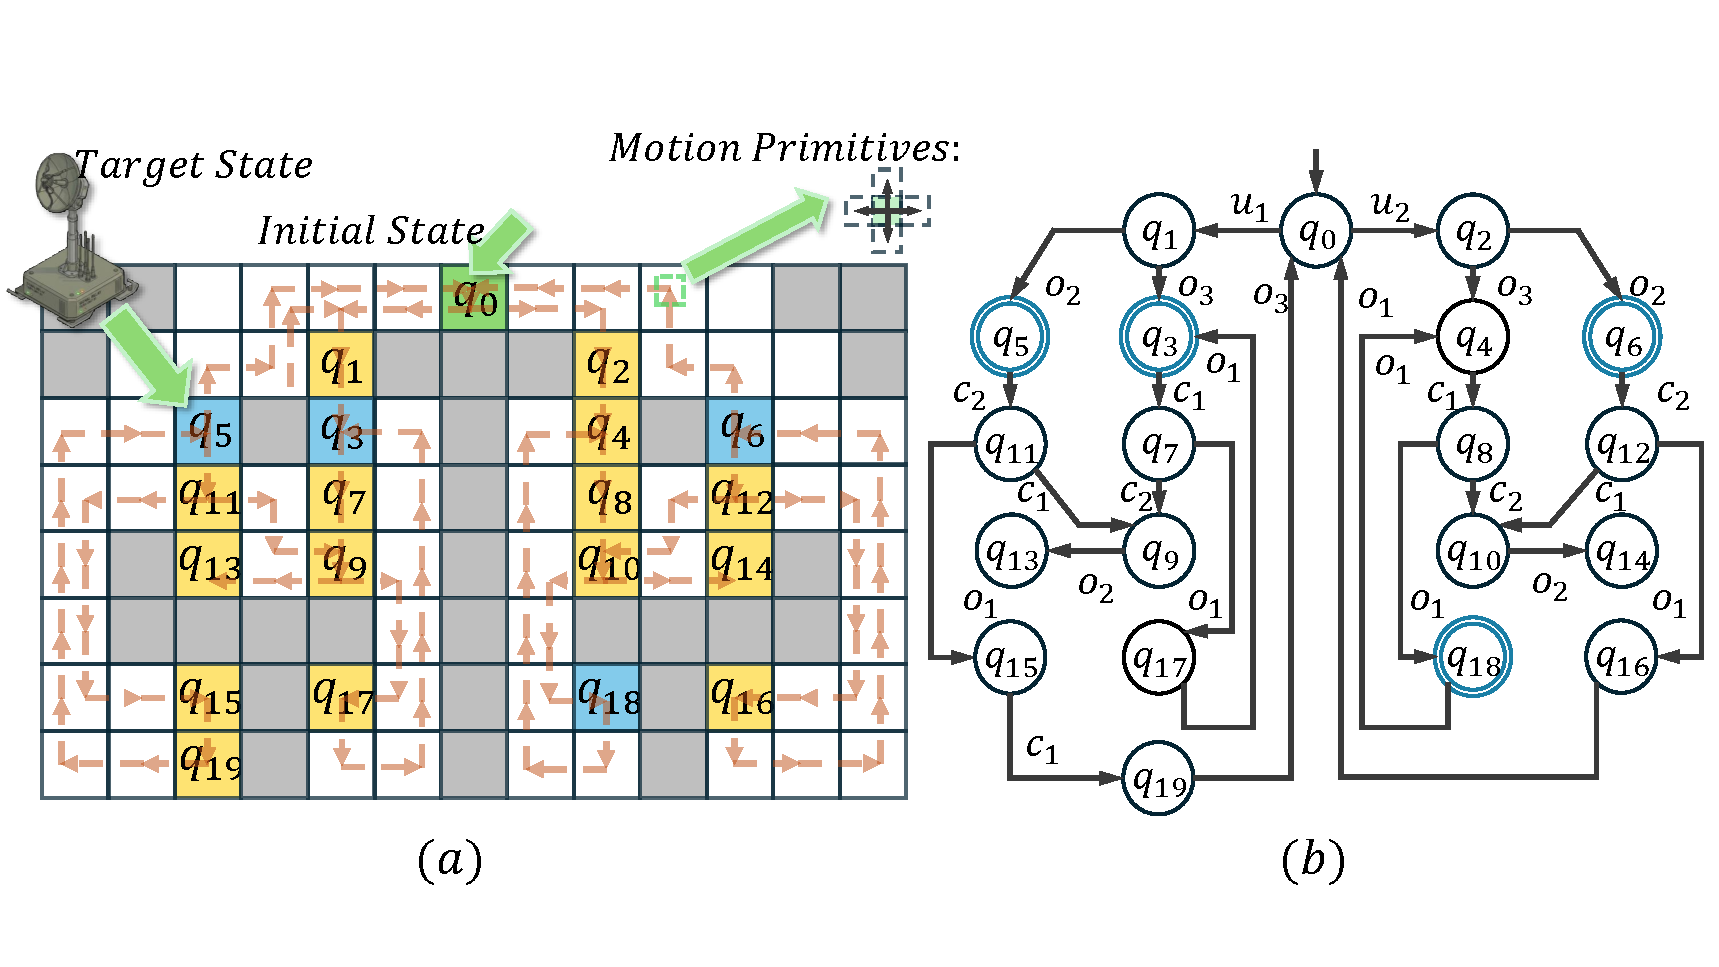
\includegraphics[width=\linewidth]{Figs/Grid_Environment_DFA.pdf}
    \caption{Deterministic finite state automaton $G$ constructed from the motivating example of the robotic system deployed in a partially observable environment from Section~\ref{sec:intro}, where the set of marked states $Q_m = \{ q_3, q_5, q_6, q_{18} \}$, the set of observable events $\Sigma_o = \{ o_1, o_2, o_3 \}$, and the set of controllable events $\Sigma_c = \{ c_1, c_2, o_3 \}$.}
    % \textcolor{red}{not good, the feasible transitions in (a) are not fully captured by (b), e.g., 19 $\to$ 13, 19 $\to$ 15..., maybe show them separately or motivate the paper only use words}
    %
    % Thanks for your comment
    %
    \label{fig:dfa_grid_env}
\end{figure}

\begin{mydef}[Detectable Non-Blockingness]
\label{def:cnb}
Let $G = (Q, \Sigma, \delta, q_0, Q_m)$ be a DES, let $\Sigma_o \subseteq \Sigma$ be the set of observable events, and let $S$ be a partial-observation supervisor.
The closed-loop system $S/G$ is said to be \emph{detectable non-blocking} with respect to $\Sigma_o$ and $Q_m$ if
\begin{equation}\label{eq:dect-def}
    \forall s\in \L(S/G),\exists t\in \L(S/G)/ t:\hat{\mathcal{E}}_S(P(st)) \subseteq Q_m.
\end{equation} 
\end{mydef}

Compared with standard non-blockingness, detectable non-blockingness requires more than the existence of a continuation to a marked state. It further requires that, after some feasible continuation, the supervisor can determine from its observation that the current state estimate is entirely contained in the marked-state set. In other words, task completion must not only be reachable in the plant, but also eventually detectable from the observation.

Clearly, detectable non-blockingness implies standard non-blockingness.
Indeed, if \eqref{eq:dect-def} holds, then for every reachable behavior $s \in \mathcal{L}(S/G)$, there exists a feasible continuation $t$ such that the state estimate after observing $P(st)$ satisfies $\hat{\mathcal{E}}_S(P(st)) \subseteq Q_m$.
Since the actual plant state consistent with this observation belongs to the estimate, the system has reached a marked state at this detection instant. 
However, the converse is not true, i.e.,  a closed-loop system may be non-blocking while failing to be detectable non-blocking.
% TODO
%\XY{give a short counter example in Figure}
%
\begin{myexm}\label{ex:counter_ex}
    Consider the DFA $G$ shown in Fig.~\ref{fig:counter_example}.
    It is straightforward to verify that $G$ is non-blocking, since every reachable state can be extended to one of the marked states $q_1$ or $q_6$.
    However, $G$ is not detectable non-blocking.
    Consider two strings $s_1$ and $s_2$ that generate the same observation
    $\alpha = o_1 o_2$, but reach different states:
    $$
        \delta(q_0,s_1)=q_5,
        \qquad
        \delta(q_0,s_2)=q_6.
    $$
    Since $q_6\in Q_m$ whereas $q_5\notin Q_m$, the immediate state estimate after observing $\alpha$ is
    $$
        \hat{\mathcal{E}}_S(\alpha)=\{q_5,q_6\}\not\subseteq Q_m.
    $$
    Although the system can physically reach a marked state, the supervisor cannot determine from the observation $\alpha$ whether the current state is marked.
    %Therefore, this DFA satisfies standard non-blockingness but violates detectable non-blockingness.
\end{myexm}
%
Based on Example~\ref{ex:counter_ex}, the proposed notion is strictly stronger than standard non-blockingness.
%
We now formulate the detectably non-blocking supervisory control problem.


\begin{figure}[ht]
    \centering
    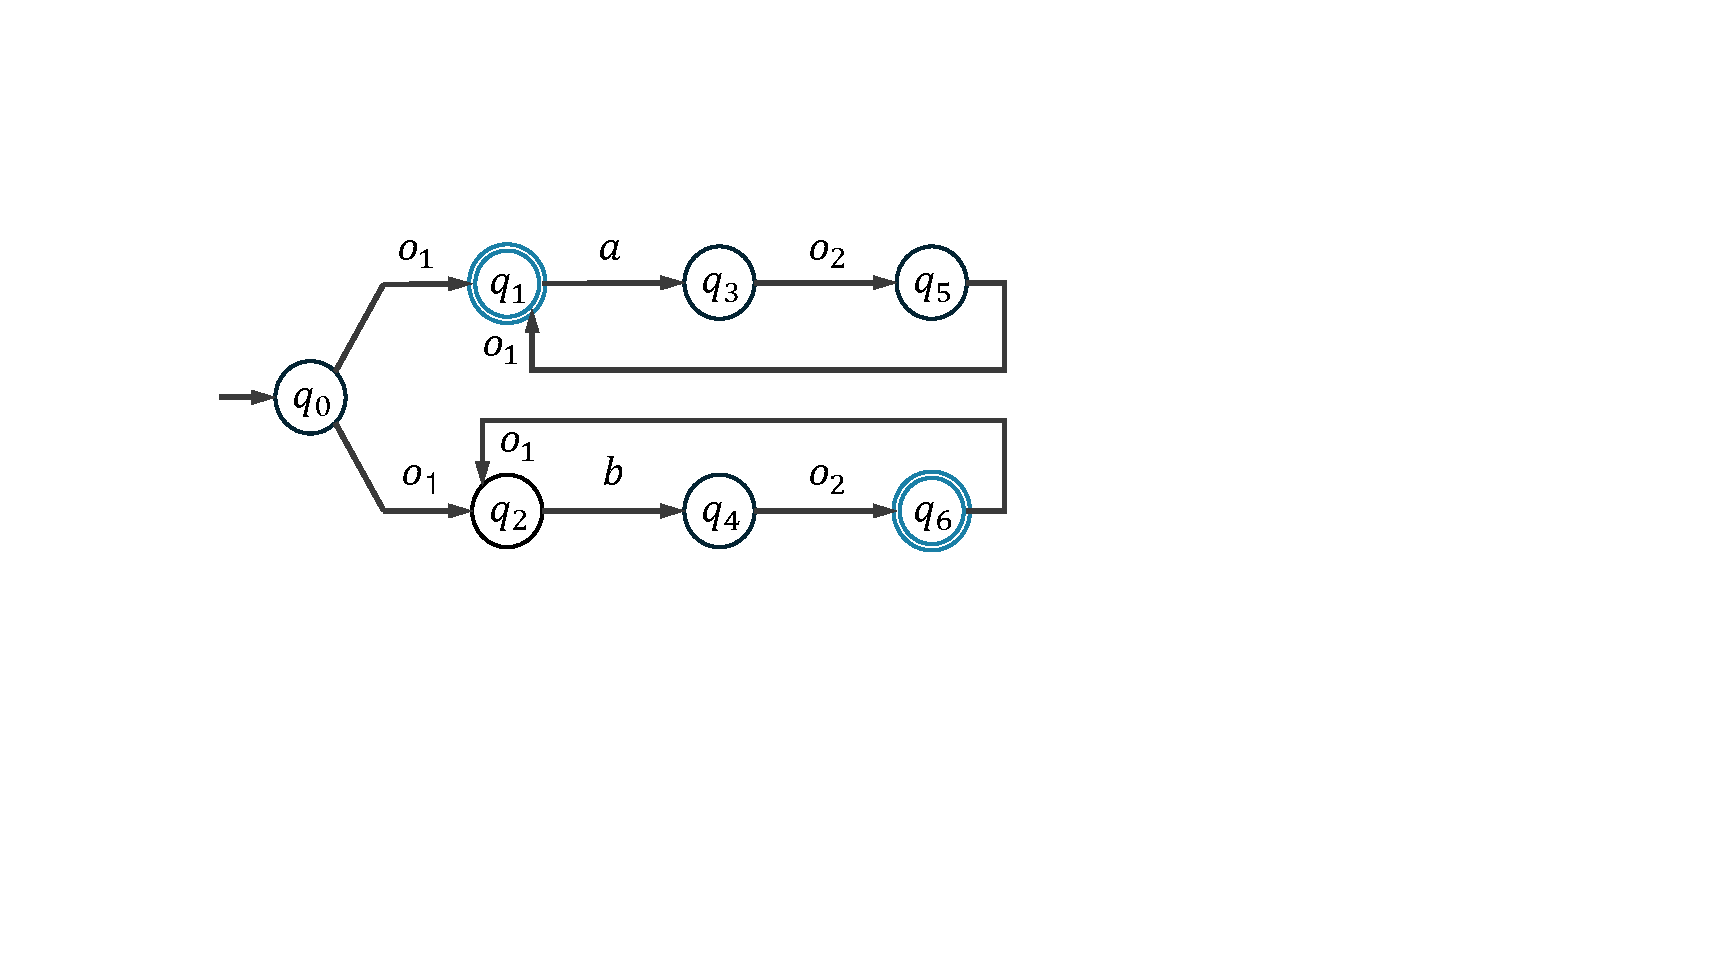
\includegraphics[width=0.65\linewidth]{Figs/counter_example_nb.pdf}
    \caption{A counterexample DFA $G$ that satisfies standard non-blockingness but violates detectable non-blockingness, where the observable event set $\Sigma_o = \{ o_1, o_3 \}$, and the marked state set $Q_m = \{ q_1, q_6 \}$.}
    \label{fig:counter_example}
\end{figure}


% TODO
% detectable -> detectable?
% should we replace all ``detectable'' to ``detecable''
\begin{myprob}%[Detectably Non-Blocking Supervisory Control]
\label{prob:cnb}
\textbf{\textup{(Detectably Non-Blocking Supervisory Control)}}
Given a DES $G = (Q, \Sigma, \delta, q_0, Q_m)$, an observable event set $\Sigma_o \subseteq \Sigma$, and a controllable event set $\Sigma_c \subseteq \Sigma$, synthesize a partial-observation supervisor $S$ such that:
\begin{enumerate} 
\item the closed-loop system $S/G$ is detectably non-blocking with respect to $\Sigma_o$ and $Q_m$;
\item $S$ is maximally permissive among all supervisors satisfying item~(i), i.e., there does not exist another supervisor $S'$ satisfying item~(i) such that
$\mathcal{L}(S/G) \subsetneq \mathcal{L}(S'/G).$
\end{enumerate}
\end{myprob}
\medskip 

\begin{remark}
In Definition~\ref{def:cnb}, detectability is formulated using the immediate state estimate $\hat{\mathcal{E}}_S(\alpha)$ rather than the state estimate with unobservable tails $\mathcal{E}_S(\alpha)$.
For any observation $\alpha \in \Sigma_o^*$, we have $\hat{\mathcal{E}}_S(\alpha) \subseteq \mathcal{E}_S(\alpha)$ 
because $\mathcal{E}_S(\alpha)$ additionally includes states that may be reached through unobservable events after the last observed event.
Therefore, using $\hat{\mathcal{E}}_S(\alpha)$ gives a more relaxed notion of detectable non-blockingness.
Intuitively, this means that the system evaluates whether it has detectably reached a marked state immediately when a new observable event is received.
Throughout this paper, we focus on the formulation based on $\hat{\mathcal{E}}_S(\alpha)$.
Nevertheless, the proposed method can be adapted to the stronger condition $\mathcal{E}_S(\alpha) \subseteq Q_m$, where task completion must remain detectable even after possible unobservable tails.
This extension will be discussed in Section~\ref{sec:special_z_marked}.
\end{remark}
 


\subsection{Challenge of the synthesis problem}

\begin{figure}[t]
    \centering
    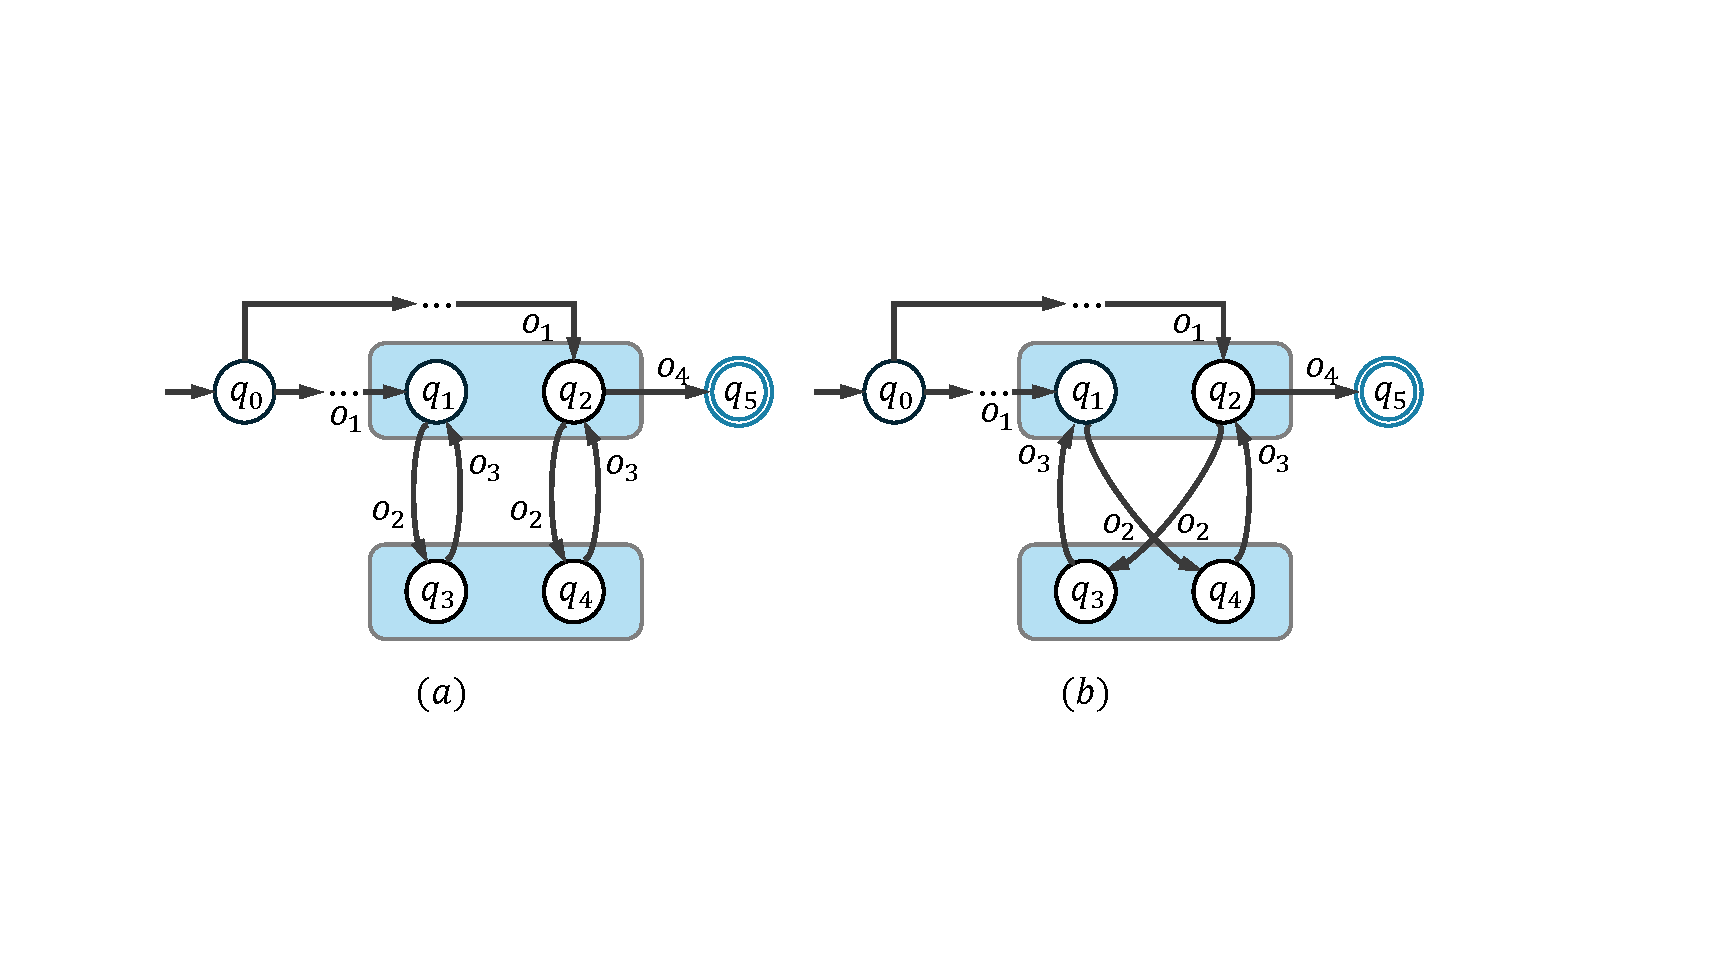
\includegraphics[width=\linewidth]{Figs/obs_nb_challenge.pdf}
    \caption{The DFAs $G_1$ and $G_2$ are shown in subfigures~(a) and~(b), respectively, with observable event set $\Sigma_o = \{ o_1, o_2, o_3, o_4\}$ and marked-state set $Q_m = \{ q_5 \}$. 
    The shaded regions represent identical observation-induced state estimates, and the corresponding estimate transitions are the same in both systems, showing that $G_1$ and $G_2$ induce the same observer-level structure. 
    $G_1$ is blocking because $q_1$ and $q_3$ are not co-accessible to $q_5$, whereas $G_2$ is non-blocking owing to its cross-coupled transitions.}
    \label{fig:obs_nb_challenge}
\end{figure}

A central challenge is that non-blockingness is not determined by the observer-level structure alone.
An observer captures how state estimates evolve under observable events, but it does not retain the internal transition connectivity among the concrete states in each estimate.
Since non-blockingness requires every reachable state to admit a continuation to a marked state, an observer state may appear co-accessible even though some of its constituent states are blocking.
The following example illustrates this mismatch between the observer-based structure and state-level non-blocking co-accessibility.



\begin{myexm}\label{ex:obs_nb_challenge_cnb}
Consider the two DFAs $G_1$ and $G_2$ in Fig.~\ref{fig:obs_nb_challenge}, with observable event set
$
    \Sigma_o = \{ o_1, o_2, o_3, o_4 \}
$
and marked-state set
$
    Q_m=\{ q_5 \}.
$
One can easily check that both systems induce the same observation-based estimates $\{ q_1, q_2 \}$ and $\{ q_3, q_4 \}$.
For simplicity, we omit the co-accessibility of states $q_0$ and the intermediate states between $q_0$ and $q_1$, or $q_0$ and $q_2$, and only discuss the non-blocking property of states $q_0$ to $q_5$ in place of the overall system.
%
For DFA $G_1$ of Fig.~\ref{fig:obs_nb_challenge} (a), since states $q_1$ and $q_3$ are not co-accessible to the marked state $q_5$, the system violates the non-blocking property.
In contrast, the cross-coupled transitions in DFA $G_2$ of Fig.~\ref{fig:obs_nb_challenge} (b) ensure that every state can eventually reach $q_5$ via the transition sequence $q_3 \xrightarrow{o_3} q_1 \xrightarrow{o_2} q_4 \xrightarrow{o_3} q_2 \xrightarrow{o_4} q_5$, and hence $G_2$ is non-blocking.
\end{myexm}

Example~\ref{ex:obs_nb_challenge_cnb} shows that identical observer-level structures may correspond to different non-blocking properties.
We next use the same pair of DFAs to explain why the observer-level structure alone is also insufficient for detectably non-blocking synthesis under partial observation.

\begin{myexm}\label{ex:obs_based_structure_insufficient}
Consider again the two DFAs $G_1$ and $G_2$ in Fig.~\ref{fig:obs_nb_challenge}.
Because they induce the same observer-level structure, any synthesis method whose input is restricted to this structure receives identical information for both systems.
%
Restricting attention to states $q_1$ through $q_5$, the observer consists of the states $\{q_1, q_2\}$, $\{q_3, q_4\}$, and $\{q_5\}$ with transitions
$
\{q_1,q_2\} \xrightarrow{o_2} \{q_3,q_4\},
\{q_3,q_4\} \xrightarrow{o_3} \{q_1,q_2\},
\{q_1,q_2\} \xrightarrow{o_4} \{q_5\}.
$
At the observer level, $\{q_1, q_2\}$ appears co-accessible because of the $o_4$-transition enabled by $q_2$.
However, non-blocking synthesis requires that such apparent progress at the estimate level be realizable from every underlying state consistent with the estimate under observation-consistent control decisions.

Classical methods such as backward reachability search~\cite{thuijsman2020transformational,thuijsman2024reducing} or the bipartite all-inclusive controller~\cite{yin2016synthesis} operate solely on partial-observation state estimates or on their aggregated reachability graphs.
%
Consequently, they cannot decide whether individual states such as $q_1$ or $q_3$ should be pruned without additional DFA-state-level transition information.

\end{myexm}

Examples~\ref{ex:obs_nb_challenge_cnb} and~\ref{ex:obs_based_structure_insufficient} reveal that the observer fails to capture the coupling between observer-level estimation and concrete state-level reachability, which is essential for non-blockingness.
%
Moreover, in detectably non-blocking synthesis, after every observation-consistent decision history, each state contained in the current observer-level estimate must admit a continuation that is consistent with the induced observer-level evolution and eventually reaches a set of states that can be certified as a subset of the marked states $Q_m$.

This requirement cannot be satisfied using the observer alone, since it discards the internal transition structure within each estimate.
%
Accordingly, Problem~\ref{prob:cnb} requires a structure that simultaneously tracks both the evolution of observation-induced estimates and the underlying DFA-state-level transitions that realize such evolution.
%
Such a structure must explicitly maintain the interaction between these two levels, so that observer-level evolution and state-level reachability can be evaluated in a unified manner.
 

% ---------------------------------------------------------------------------------
\section{Inter-connected bipartite transition system}\label{sec:bcc}

In this section, we attempt to solve the detectably non-blocking problem using information-state-based structures.
%
We first give the notion of information state and the corresponding update rules to represent both unobservable reach under control patterns and observable reach with respect to specific observations.
%
We then put forward the inter-connected bipartite transition system (IC-BTS) that captures the microscopic evolution of the information states.


\subsection{System definition and construction}


Based on the update rules defined in \eqref{eq:ur} and \eqref{eq:nx}, we need a structure that can not only track the evolution of the controlled system based on the partial observations, but also track the microscopic structure within unobservable reaches and observable reaches.
%
The inter-connected bipartite transition system (IC-BTS) structure fulfills this role by expanding information states and recording admissible control sequences.
Now, we give the formal definition of IC-BTS as follows.
%

\begin{mydef}\label{def:bcc}
Given a DFA $G$, its corresponding IC-BTS is a tuple
$
\mathfrak{S} = (\hat{\mathbb{I}}, \mathbb{I}, \hat{\imath}_0, \Sigma, \Gamma, \delta_{DO}, \delta_{OO}, \delta_{OD})
$
where
\begin{enumerate}[(i)]
    \item 
    $\hat{\mathbb{I}} \subseteq Q \times 2^Q$ is the set of  \emph{decision states}, 
    where $\hat{\imath}_0 = ( q_0,\{ q_0 \}) \in \hat{\mathbb{I}}$ is the initial state; 
    \item 
    $\mathbb{I}  \subseteq Q \times 2^Q\times \Gamma$ is the set of  \emph{observation states};
    \item 
    $\Sigma$ is the set of events in $G$;
    \item
    $\Gamma \subseteq 2^{\Sigma}$ is the set of control patterns; 
    \item 
    the transition function has three different types: 
    
    $\delta_{DO} : \hat{\mathbb{I}} \times \Gamma \rightarrow \mathbb{I}$ is the partial transition function from decision states to observation states, such that, for any
    $\hat{\imath} = (\hat{q}, \hat{x}) \in \hat{\mathbb{I}}$, 
    $\imath = ({q}, {x},\gamma) \in {\mathbb{I}}$,
    we have $\delta_{DO}(\hat{\imath},\gamma)=\imath$ only if 
    \begin{equation}
        [q=\hat{q}] \wedge [{x} = UR_{\gamma}(\hat{x})];
    \end{equation}
    
    $\delta_{OO} : \mathbb{I} \times \Sigma_{uo} \rightarrow \mathbb{I}$ is the partial transition between observation states, such that, for any
    $\imath = ({q}, {x},\gamma),\imath' = ({q}', {x}',\gamma')  \in {\mathbb{I}},\sigma\in\Sigma_{uo}\cap\gamma$,
    we have $\delta_{OO}({\imath},\sigma)=\imath'$ only if 
    \begin{equation}
        [q'=\delta(q,\sigma)] \wedge [x'=x]  \wedge [\gamma'=\gamma];
    \end{equation}

    \item $\delta_{OD} : \mathbb{I} \times \Sigma_o \rightarrow \hat{\mathbb{I}}$ is the partial transition function from observation states to decision states, such that for $\hat{\imath} = (\hat{q}, \hat{x}) \in \hat{\mathbb{I}}$, $\imath = ({q}, {x},\gamma) \in {\mathbb{I}}$, we have $\hat{x} = NX_{\sigma}({x})$ for $\sigma \in \gamma \cap \Sigma_o$.

    % 
    % \hat{\mathbb{I}}_m 要在后续被定义
    
\end{enumerate}
\end{mydef}
%
For each $x\in 2^Q$, we define 
\[
\hat{\mathbb{I}}(x)=\{ (q,x)\in Q\times 2^Q\mid q\in x \}.
\]
For each $x\in 2^Q,\gamma\in \Gamma$, we define 
\[
{\mathbb{I}}(x,\gamma)=\{ (q,x,\gamma)\in Q\times 2^Q\mid q\in x \}.
\]
%
% TODO, 这个用法争取在后续不再使用
%       转为分开定义a run rho ends at control / decision states
%   In IC-BTS $\mathfrak{S}$, we use $P = Y \cup Z$ to denote the set of states.
%
% TODO
% 这个也不再使用
% For a decision state $y = (x_y, q_y)$ and an observation state $z = (x_z, q_z, \gamma_z)$, we further denote
% $X(y) = q_y$, $X(z) = q_z$, $Q(y) = q_y$, $Q(z) = q_z$, and $\Gamma(z) = \gamma_z$.

The run (state event sequence) in IC-BTS $\mathfrak{S}$ is of the following form
\begin{equation}\label{eq:run_bcc}
\begin{aligned}
&\rho = \\
{}&
\begin{array}[t]{@{}l@{}}
\hat{\imath}_0
\xrightarrow{\gamma_0} {\imath}_{1,1}
\xrightarrow{\sigma_{u}^{(1,1)}} {\imath}_{1,1}
\xrightarrow{\sigma_{u}^{(1,2)}} {\imath}_{1,2}
\cdots
\xrightarrow{\sigma_{u}^{(1,m_1)}} {\imath}_{1,m_1}
\\[0.6em]
\xrightarrow{\sigma_{o}^{(1)}} \hat{\imath}_1
\xrightarrow{\gamma_1} {\imath}_{2,1}
\xrightarrow{\sigma_{u}^{(2,1)}} {\imath}_{2,1}
\xrightarrow{\sigma_{u}^{(2,2)}} {\imath}_{2,2}
\cdots
\xrightarrow{\sigma_{u}^{(2,m_2)}} {\imath}_{2,m_2}
\\[0.4em]
\multicolumn{1}{c}{\vdots}
\\[0.4em]
\xrightarrow{\sigma_{o}^{(k)}} \hat{\imath}_k
\xrightarrow{\gamma_k} {\imath}_{k,1}
\xrightarrow{\sigma_{u}^{(k,1)}} {\imath}_{k,1}
\xrightarrow{\sigma_{u}^{(k,2)}} {\imath}_{k,2}
\cdots
\xrightarrow{\sigma_{u}^{(k,m_k)}} {\imath}_{k,m_k},
\end{array}
\end{aligned}
\end{equation}
such that the sequences
\begin{flalign}
\rho\restriction_{\imath} &= 
\hat{\imath}_0 {\imath}_{1,1} {\imath}_{1,2} \cdots {\imath}_{1,m_1} \hat{\imath}_1 {\imath}_{2,1}{\imath}_{2,2} \cdots
\label{eq:seq_bcc:i} \\
%
\rho\restriction_{\delta} &=  \gamma_0 \sigma_{u}^{(1,1)} \sigma_{u}^{(1,2)} \cdots \gamma_1 \sigma_{u}^{(2,1)} \cdots
\label{eq:seq_bcc:delta} \\
%
\rho\restriction_{X}      &= \hat{x}_0 (x_0, \gamma_0) \hat{x}_1 (x_1, \gamma_1) \cdots
\label{eq:seq_bcc:X}
\end{flalign}
are for the state sequence, control-event sequence, and macrostate sequences,
and
$\hat{x}_0$, $(x_1, \gamma_1)$, $\hat{x}_1 $, and $(x_2, \gamma_2)$ denote the macrostates of $\hat{\imath}_0 = (q_0, x_0)$, $\imath_{1,j} = (q_{1,j}, x_1, \gamma_1)$, $\hat{\imath}_1 = (\hat{q}_1, \hat{x}_1)$, and $\imath_{2,j} = (q_{2,j}, x_2, \gamma_2)$, respectively.
%
%
% 为什么是o? 因为这是能看见的
% TODO
% follow this idea such that the notations can be simple and instant reasoning
% \[
% \rho\restriction_{o}= 
% \hat{\imath}_0{\imath}_{1,1}\hat{\imath}_1{\imath}_{2,1}
% \dots 
% \hat{\imath}_k{\imath}_{k,1}..?
% \]
%
%
Intuitively, the IC-BTS structure is introduced to describe the ``game'' between the supervisor and the system under partial observation. 
%
It represents not only the control-observation evolution at the level of information states, but also the microscopic transitions within each information state.
The decision states represent sets of observation-equivalent states and serve as decision-making instances for the supervisor, whereas the observation states represent the resulting information states together with the selected decision $\gamma$, from which the system resolves the next observable event.
%
The transition from $\hat{\imath} \xrightarrow{\gamma} \imath$ captures the unobservable reach under decision $\gamma$,
The transition $\imath \xrightarrow{\sigma_{u}} \imath'$ captures the transitions within an unobservable reach,
and the transition $\imath \xrightarrow{\sigma_o} \hat{\imath}'$ captures the observable reach after an event $\sigma_o \in \Sigma_o$.
%
Moreover, to specify the control and evolution of the original DFA, we extract the event sequence and control pattern sequence, respectively, from \eqref{eq:run_bcc} -- \eqref{eq:seq_bcc:X} as follows,
\begin{flalign}
    \rho\restriction_{\sigma} &= \sigma_{u}^{(1,1)} \cdots \sigma_{u}^{(1,m_1)} \sigma_{o}^{(1)}\sigma_{u}^{(2,1)} \cdots \label{eq:seq_bcc:sigma} \\
    \rho\restriction_{\gamma} &= \gamma_0 \gamma_1 \cdots \gamma_i. \label{eq:seq_bcc:gamma}
\end{flalign}
%



\begin{algorithm2e}[t]
\caption{Construction of IC-BTS}
\label{alg:bcc}

\Indentp{-1.25em}
\KwIn{DFA $G=(Q,\Sigma,\delta,q_0,Q_m)$ with event partitions
      $\Sigma=\Sigma_c\dot{\cup}\Sigma_{uc}=\Sigma_o \dot{\cup} \Sigma_{uo}$\;}
\KwOut{IC-BTS $\mathfrak{S} = (\hat{\mathbb{I}}, \mathbb{I}, \hat{\imath}_0, \Sigma, \Gamma, \delta_{DO}, \delta_{OO}, \delta_{OD})$\;}
\Indentp{1.25em}

Initialize $\Gamma = \{\gamma\in 2^\Sigma \mid \Sigma_{uc}\subseteq \gamma \}$, $\hat{\imath}_0 = (q_0, \{q_0\})$\;

\ForEach{unprocessed decision macrostate $\hat{x}$}{                   % TODO
    % Include all $(\hat{q}, \hat{x})$, $\forall \hat{q} \in \hat{x}$ into $\hat{\mathbb{I}}$\;
    Include $\hat{\mathbb{I}}(\hat{x})$ into $\hat{\mathbb{I}}$;

    % \tcp{Enumerate all control patterns for all-inclusive construction}
    \ForEach{control pattern $\gamma \in \Gamma$}{
        Generate observation macrostate $(x, \gamma)$, for $x \gets UR_{\gamma}(\hat{x})$\;
        
        % Include all observation states $(q, x, \gamma)$, $\forall q \in x$\;
        Include $\mathbb{I}(x,\gamma)$ into $\mathbb{I}$;
        
        Add decision-observation transitions $(\hat{q}, \hat{x}) \xrightarrow[]{\gamma} (q, x, \gamma)$, $\forall \hat{q} = q$\;  % 就算$q_y$有自循环也需要这么做
        
        Add observation-observation transitions $(q, x, \gamma) \xrightarrow[]{\sigma_{u}} (q', x, \gamma)$, $\forall q \xrightarrow[]{\sigma_{u}} q'$\;

        \ForEach{observable event $\sigma_o \in \gamma \cap\Sigma_o$}{    % TODO 这个说法改一下, 我觉得前面的remark得留下来说明这个事, 不然一直很别扭
            Compute $\hat{x}' = NX_{\sigma_o}(x)$\;
            
            % Include $(\hat{q}', \hat{x}')$ $\forall \hat{q}' \in \hat{x}'$ and add observation-decision transitions $(q, x, \gamma) \xrightarrow[]{\sigma_o} (\hat{q}', \hat{x}')$\;
            Include $\hat{\mathbb{I}}(\hat{x}')$ into $\hat{\mathbb{I}}$ and add observation-decision transitions $(q, x, \gamma) \xrightarrow[]{\sigma_o} (\hat{q}', \hat{x}')$\;

            Enqueue $\hat{x}'$ if it has not been processed\;
        }
    }
}

% Set $\mathbb{I}_m = \{ (q, x) \in \mathbb{I} \mid x \subseteq Q_m \}$ and $\Sigma_{\mathfrak{S}} \gets \Sigma \cup \Gamma$\;

\Return $\mathfrak{S}$\;
\end{algorithm2e}
%
We give Algorithm~\ref{alg:bcc} for the construction of an IC-BTS from the original DFA $G$.
Algorithm~\ref{alg:bcc} follows a breadth-first search (BFS) structure.
It iteratively computes all successor observation macrostates from each decision macrostate under all admissible control patterns, and then derives successor decision macrostates from the observable projections of the newly generated observation macrostates.
Meanwhile, whenever a new macrostate is generated, the algorithm also constructs the associated decision and observation states, together with the transition relations induced by the underlying DFA transitions.
%
In Lines 2--7, the algorithm explores decision macrostates in a BFS manner.
For each decision macrostate $\hat{x}$, it adds all corresponding decision states $(\hat{q}, \hat{x})$ with $\hat{q} \in \hat{x}$ into the IC-BTS, and enumerates all control patterns to compute successor observation macrostates via the operator $\UR(\cdot)$.
% The corresponding decision-observation micro-transitions, which correspond to the selected control decision, are then added to the IC-BTS in Line 7.
%
In Line 8, the algorithm expands each newly generated observation macrostate by adding all observation states $(q, x, \gamma)$ and recording the internal unobservable transitions within the same observation macrostate.
%
In Lines 9--12, the algorithm computes successor decision macrostates using the operator $\NX(\cdot)$ for observable events, and adds the corresponding decision states and observation-decision transitions to the IC-BTS.
%
We use Example~\ref{ex:bcc} to illustrate the construction of IC-BTS.
%
\begin{myexm}\label{ex:bcc}
    Let us reconsider DFA $G$ in Fig.~\ref{fig:dfa_grid_env}~(b), where the observable event set is
    $\Sigma_o = \{o_1,o_2,o_3\}$ and the controllable event set is
    $\Sigma_c = \{c_1,c_2,o_3\}$.
    By applying Algorithm~\ref{alg:bcc}, we construct the corresponding IC-BTS, whose overall structure is shown in Fig.~\ref{fig:bcc_overall}.
    In this figure, orange rectangles represent decision macrostates, while blue rounded rectangles represent observation macrostates.
    For readability, we simplify the notation of macrostates from $(\hat{q},\hat{x})$ and $(q,x,\gamma)$ to $\hat{q}$ and $q$, respectively.
    We also use different colors to distinguish different branches of transition relations and omit the uncontrollable events contained in each control pattern, so as to emphasize the structural properties of the constructed IC-BTS.

    We also demonstrate the evolution of the IC-BTS as follows.
    %
    For the initial macrostate $\{ q_0 \}$, since $u_1, u_2$ are uncontrollable and unobservable, the only available control pattern is $\gamma_0 = \{ o_3 \}$.
    Next, we have $x_{1} = \{ q_0, q_1, q_2 \} = UR_{\gamma_0}(\hat{\imath}_0)$, and the corresponding observation state set is
    \[
    \mathbb{I}(x_1,\gamma_1) =
    \{(q_0,x_1,\gamma_1),(q_1,x_1,\gamma_1),(q_2,x_1,\gamma_1)\}.
    \]
    where states $q_0$, $q_1$, $q_2$ are accessible from state $q_0$ through the unobservable transitions $\epsilon$, $u_1$, and $u_2$, respectively.
    %
    For observation macrostate $(x_{1}, \gamma_1)$, the observable reach based on observation $o_3$ and $o_2$ is
    $\hat{x}_{1} = NX_{o_3}(x_{1}) = \{ q_3, q_4 \}$ and $\hat{x}_{2} = NX_{o_2}(x_{1}) = \{ q_5, q_6 \}$, and the corresponding decision state set is
    \[
    \hat{\mathbb{I}}(\hat{x}_1)  =
    \{(q_3,\hat{x}_1),(q_4,\hat{x}_1)\}.
    \]
    %
    Similarly, based on the possible unobservable evolution $q_3 \xrightarrow{c_1} q_7 \xrightarrow{c_2} q_9$ and $q_4 \xrightarrow{c_1} q_8 \xrightarrow{c_2} q_{10}$, we can enable no event, namely $\emptyset$, or enable $\{ c_1 \}$, $\{ c_2 \}$, or $\{ c_1,c_2 \}$ at this step.
    Then, we have
    $x_{4} = UR_{\gamma_2}(x_{1}) = \{ q_3, q_4, q_7, q_8 \}$ and
    $x_{7} = UR_{\gamma_3}(x_{1}) = \{ q_3, q_4, q_7, q_8, q_9, q_{10} \}$,
    where $\gamma_2 = \{ c_1 \}$ and $\gamma_3 = \{ c_1, c_2 \}$.
    For observation macrostates $(x_{7}, \gamma_3)$, we have
    $\hat{x}_{5} = NX_{o_2}(x_{7}) = \{ q_{13}, q_{14} \}$ and
    $\hat{x}_{3} = NX_{o_1}(x_{7}) = \{ q_{17}, q_{18} \}$.
\end{myexm}



%
\begin{figure*}[t!]
    \centering
    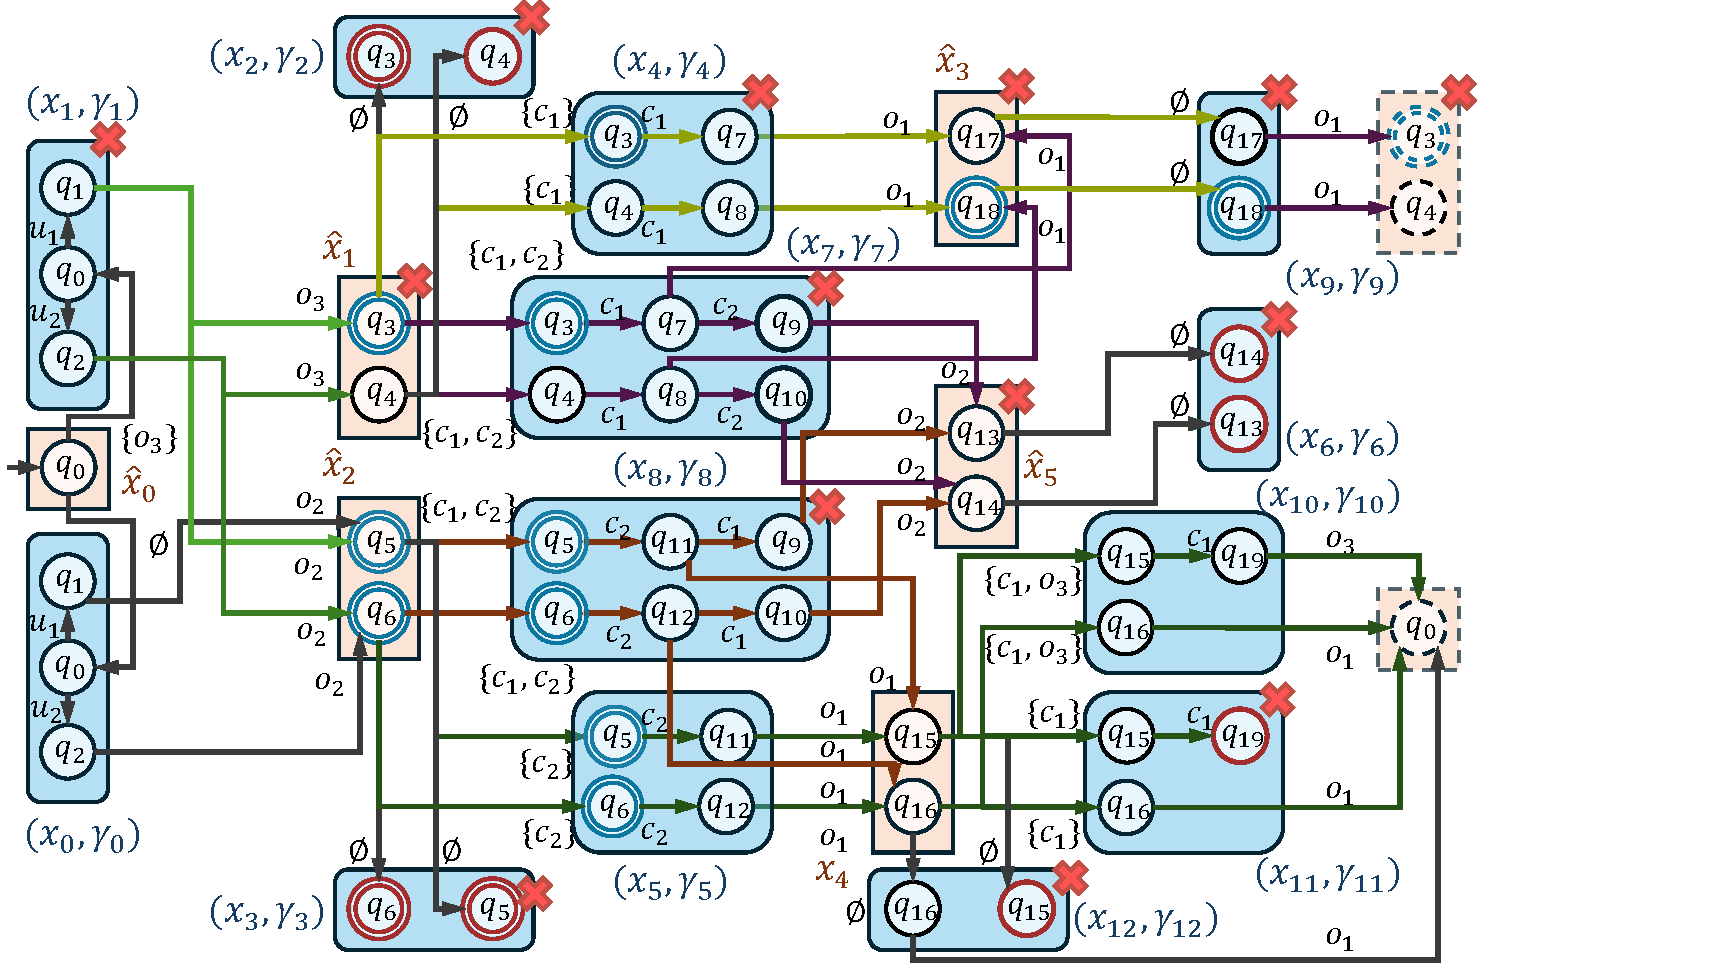
\includegraphics[width=0.615\linewidth]{Figs/bcc_overall_2.pdf}
    \caption{Inter-connected bipartite transition system constructed from the DFA $G$ in Fig.~\ref{fig:dfa_grid_env} (b). We simplify the notations $(\hat{q}, \hat{x})$ and $(q, x, \gamma)$ to $\hat{q}$ and $q$, respectively, and omit the uncontrollable events contained in each control pattern to better illustrate the structural properties of each state.
    Orange rectangles represent decision macrostates, while blue rounded rectangles represent observation macrostates.
    Transitions in different colors are used to distinguish different evolutions. Moreover, the information states marked by red crosses are infeasible observation macrostates, detectably blocking decision macrostates, or inconsistent decision or observation macrostates, which should be pruned to achieve detectable non-blocking.
    The source code is available at \protect\url{https://github.com/trigger1996/des_common/tree/master/detectable_nonblocking}.}   % TODO, 最好拆成几个库
    \label{fig:bcc_overall}
\end{figure*}


\subsection{Properties of inter-connected bipartite transition system}

%
% 这段是重复的
% The IC-BTS represents the system evolution at two levels: the macrostate level and the DFA-state level. 
% At the macrostate level, it captures the evolution induced by partial observations and control decisions. 
% At the DFA-state level, it records the detailed transitions among individual DFA states, including internal transitions within unobservable reaches and observable transitions between decision or observation states.
%
%
% Based on the above notations, we analyze the properties of the IC-BTS, illustrating the consistency of its evolution with the original DFA, the completeness of the control representation, and its construction complexity in terms of both time and space.
% %
% % We first clarify a structural restriction on decision macrostates. 
% Recall that decision macrostates represent observation-equivalent states under supervisory control, and thus transitions between decision states must preserve the observation structure. In particular, for any $\hat{\imath}, \hat{\imath}' \in \hat{\mathbb{I}}$, we have
% $
% (\hat{\imath}, \eta, \hat{\imath}') \notin \delta_{\mathfrak{S}}, \forall \eta \in \Sigma_{\mathfrak{S}}.
% $
%
% Building on this restriction, we describe the internal structure of observation macrostates $(x, \gamma)$ and their corresponding observation state $\imath \in \mathbb{I}$.
%
%
%
% For an entry observation state $\imath = (q, x, \gamma)$ and any predecessor decision state $\hat{\imath} = (\hat{q}, \hat{x})$, since $\epsilon$ is admissible to be the transition from $\hat{\imath}$ to $\imath$ at the DFA state level, we have $q \in \hat{\imath} \cap \imath$.
% This shows that observation states inherit their information state from decision states under unobservable transitions.
%
% Moreover, transitions within an observation macrostate are induced by an unobservable reach $\UR(\cdot)$ starting from its predecessor decision macrostates.
% %
% % Therefore, reachability within an observation state is consistent with this inheritance structure. 
% Specifically, for any entry observation state $\imath = (q, x, \gamma)$ and its predecessor decision state $\hat{\imath}$, every $\imath' \in x$ is reachable via a string 
% $
% s \in (\gamma \cap \Sigma_{uo})^*
% $ 
% such that
% $$
% (q,  x, \gamma) = \delta_{\mathfrak{S}}((q, \hat{x}), \gamma),
% \quad
% (q', x, \gamma) = \delta_{\mathfrak{S}}((q, x, \gamma), s).
% $$
% %
% We give the following proposition to illustrate the consistency between the DFA $G$ and the IC-BTS $\mathfrak{S}$.
%



The IC-BTS represents the system evolution at two levels: the macrostate level and the DFA-state level. 
At the macrostate level, it captures the evolution induced by partial observations and control decisions. 
At the DFA-state level, it records the detailed transitions among individual DFA states, including internal transitions within unobservable reaches and observable transitions between observation and decision states.
%
By Definition~\ref{def:bcc}, the decision-observation transition
$\hat{\imath}_{k-1} \xrightarrow{\gamma_{k-1}} \imath_{k,1}$
selects the control pattern $\gamma_{k-1}$ and starts the corresponding unobservable reach, rather than generating an actual transition of $G$.
The observation-observation transition
$\imath_{k,j} \xrightarrow{\sigma_u^{(k,j)}} \imath_{k,j+1}$
records the internal DFA evolution
$q_{k,j+1} = \delta(q_{k,j},\sigma_u^{(k,j)})$
under the unobservable event
$\sigma_u^{(k,j)} \in \gamma_{k-1}\cap\Sigma_{uo}$ permitted by supervisor and control pattern $\gamma_k$.
Moreover, the observation-decision transition
$\imath_{k,m_k} \xrightarrow{\sigma_o^{(k)}} \hat{\imath}_{k}$
occurs when the enabled observable event
$\sigma_o^{(k)}\in\gamma_{k-1}\cap\Sigma_o$
is observed, leading to the DFA transition
$\hat{q}_{k} = \delta(q_{k,m_k},\sigma_o^{(k)})$
and updating the decision state.
%
Hence, the event sequence $\rho\restriction_{\delta}$ can exactly represent the event sequence generated by the DFA-level transitions.
The following proposition shows that this sequence is a valid execution of the closed-loop system $S / G$.
%
\begin{mypro}
\label{prop:bcc_dfa_consistency}
Given a run $\rho$ of the IC-BTS $\mathfrak{S}$ of the form \eqref{eq:run_bcc}, let
$\rho\restriction_{\imath}$ be its state sequence defined in \eqref{eq:seq_bcc:i}.
Then there exists a corresponding string
$$
s = \xi_0\,\sigma_o^{(0)}\,\xi_1\,\sigma_o^{(1)}\,\cdots\xi_k\,\sigma_o^{(k)}\cdots\in \mathcal{L}(S/G),
$$
where
$$
\xi_k = \sigma_u^{(k,1)}\sigma_u^{(k,2)}\cdots\sigma_u^{(k,m_k)}\in(\gamma_k\cap\Sigma_{uo})^*,
$$
such that, for every $k\geq 0$, the following conditions hold:
\begin{enumerate}[(i)]
    \item for each observation-observation transition, there exists
    $\sigma_u^{(k,j)} \in \gamma_k\cap\Sigma_{uo}$ such that
    $$
        q_{k,j} = \delta(q_{k,j-1},\sigma_u^{(k,j)}), j = 1, \ldots, m_k;
    $$

    \item for each observation-decision transition, there exists
    $\sigma_o^{(k)} \in \gamma_k\cap\Sigma_o$ such that
    $$
        \hat q_{k+1} = \delta(q_{k,m_k},\sigma_o^{(k)}).
    $$
\end{enumerate}
\end{mypro}
%
As a direct consequence of Proposition~\ref{prop:bcc_dfa_consistency}, 
for events $\sigma_u^{(k,j)}$ or $\sigma_o^{(k)}$, the transition in the IC-BTS agrees with the corresponding transition in DFA, namely,
\begin{flalign}
    \imath_{k,j} = \delta_{OO}(\imath_{k,j-1}, \sigma_u^{(k,j)})
    &\Leftrightarrow
    q_{k,j} = \delta(q_{k,j-1},\sigma_u^{(k,j)}) \notag \\
    %
    \hat{\imath}_{k+1} = \delta_{OD}(\imath_{k,m_k}, \sigma_o^{(k)})
    &\Leftrightarrow
    \hat q_{k+1} = \delta(q_{k,m_k},\sigma_o^{(k)}), \notag
\end{flalign}
where $j = 1, \ldots, m_k$.    
%
Therefore, for the IC-BTS run $\rho$ defined in \eqref{eq:run_bcc}, projecting its event labels onto the DFA alphabet yields the DFA-level event sequence
\begin{equation}
    \sigma_{u}^{(1, 1)} \cdots \sigma_{u}^{(1, m_1)} \, \sigma_{o}^{(1)} \cdots
    \sigma_{u}^{(k, 1)} \cdots \sigma_{u}^{(k, m_k)} \, \sigma_{o}^{(k)} \cdots.
\end{equation}
which is feasible in $S/G$.
In other word. the IC-BTS introduces no spurious DFA behavior, but only refines feasible executions by explicitly recording control patterns, observations, and unobservable evolution.
%
% \begin{pf}
% The result follows directly from Definition~\ref{def:bcc}.
% %
% First, every observation-observation transition satisfying $\imath_{k,j} = \delta_{OO}(\imath_{k,j-1}, \sigma_{k,j})$, $j,k \in \mathbb{N}$ is defined only if $\sigma_{k,j} \in \gamma_k \cap \Sigma_{uo}$ and $q_{k,j+1} = \delta(q_{k,j}, \sigma)$, where $\gamma_k$ is defined in \eqref{eq:run_bcc}. 
% Thus, each subsequence $\imath_{i,1} \cdots \imath_{i,m_i}$ corresponds to a sequence $\xi_i \in (\gamma_i \cap \Sigma_{uo})^*$ satisfying (ii).
% %
% Second, every observation-decision transition $\imath_{k,j} \xrightarrow{\sigma_o} \hat{\imath}_{k+1}$ is defined only if $\sigma_o \in \Sigma_o$ and $\hat{q}_{k+1}' = \delta(q_{i,m_k}, \sigma_o)$ of DFA $G$, where $\imath_{k,j} = (q_{k,j}, x_{k,j}, \gamma_k)$ and $\hat{\imath}_{k+1} = (\hat{q}_{k+1}, \hat{x}_{k+1})$.
% This establishes (iii).
% %
% Finally, the decision-observation transition $\hat{\imath}_k \xrightarrow{\gamma_{k+1}} \imath_{k+1,1}$ can determine the set of admissible events $\gamma_{k+1}$ that govern the subsequent unobservable evolution within $\imath_{i+1}$, and thus constrains the corresponding subsequence $\xi_{i+1}$.
% Concatenating all such unobservable subsequences $\xi_i$ and observable events $\sigma_{o}^{(k)}$ yields a valid execution $s$ in the closed-loop system $S / G$, which proves (i).
% \end{pf}
%
% As a direct consequence of Proposition~\ref{prop:bcc_dfa_consistency}, 
% for any $\alpha \in \mathcal{L}(\mathfrak{S})$, if
% $
% \delta_{\mathfrak{S}}(\hat{\imath}_0,\alpha)=(\bm{q},q),
% $
% then
% $
%     \delta(q_0,P_\Sigma(\alpha)) = q.
% $
% In particular, we have
% $$
%     \mathcal{L}_{\Sigma}(\mathfrak{S})
%     =
%     P_\Sigma(\mathcal{L}(\mathfrak{S}))
%     \subseteq
%     \mathcal{L}(G).
% $$
% %
% This means that every event sequence generated by the IC-BTS and projected onto the DFA alphabet is feasible in $G$. Hence, the IC-BTS does not introduce any spurious DFA behavior; it only refines feasible executions of $G$ by explicitly recording the interaction among observation, control patterns, and unobservable evolution.

We next summarize the computational cost of constructing the IC-BTS. 
Since Algorithm~\ref{alg:bcc} explores decision macrostates in a breadth-first-search manner, the number of possible decision macrostates is bounded by $2^{|Q|}$. 
For each generated decision macrostate, the algorithm enumerates control patterns $\gamma \in 2^{\Sigma_c}$. 
For each pair of a decision macrostate and a control pattern, the computation of the corresponding unobservable reach, internal observation-observation transitions, and observable successors can be implemented by scanning the DFA transition table, whose cost is bounded by $O(|Q|\cdot |\Sigma|)$. Therefore, the worst-case time complexity of Algorithm~\ref{alg:bcc} is
$$
O(2^{|Q| + |\Sigma|} \cdot |Q| \cdot |\Sigma|)
$$
since $|\Sigma_c|\leq |\Sigma|$.

The size of the constructed IC-BTS is also finite. 
Each IC-BTS state is either a decision state of the form $(\hat{q}, \hat{x})$ or an observation state of the form $(q, x, \gamma)$. Since a macrostate $x$ is a subset of $Q$ and a control pattern satisfies $\gamma\in 2^{\Sigma_c}$, the total number of IC-BTS states satisfies
\begin{equation}
    \label{eq:prop:bcc:1}
    |\hat{\mathbb{I}}| + |\mathbb{I}| \leq |Q|(2^{|Q|}+2^{|Q|+|\Sigma|}).    
\end{equation}
Moreover, the transitions of the IC-BTS consist of decision-observation transitions, internal observation-observation transitions, and observation-decision transitions. Since each observation state has at most one successor under each event of the deterministic DFA $G$, the total number of IC-BTS transitions is bounded by
\begin{equation}
    \label{eq:prop:bcc:2}
    |\delta_{OD}| + |\delta_{OO}| + |\delta_{DO}| \leq |Q|\,2^{|Q|+|\Sigma|}(1+|\Sigma|).
\end{equation}
Thus, Algorithm~\ref{alg:bcc} constructs a finite IC-BTS in finite time, and both its state space and transition relation are bounded exponentially in the number of DFA states and controllable-event choices.

% That is, every DFA sequence projected from the IC-BTS is feasible and belongs to the language $\mathcal{L}(G)$.
% %
% Moreover, we provide the time complexity of Algorithm~\ref{alg:bcc} and the space complexity of IC-BTS as follows.

% \begin{mypro}
% Given a DFA $G$ with $|Q|$ states and $|\Sigma|$ events, the complexity of Algorithm~\ref{alg:bcc} in time will be dominated by
% $$
% O(2^{|Q| +|\Sigma|} \cdot (|Q|\cdot |\Sigma|))
% $$
% \end{mypro}
%
% \begin{pf}
% Algorithm~\ref{alg:bcc} performs a breadth-first search over generated decision macrostates. Since each decision macrostate is a subset of $2^Q$, the number of repetitions of Line 2 is at most
% $
%     |W^Y| \leq 2^{|Q|}.
% $
% %
% In Line 3, the decision states will be added to IC-BTS, and the repetition will be at most  $O(|Q|)$.
% %
% In Line 4, for each generated decision macrostate $w_y$, the algorithm enumerates all control patterns
% $
%     \gamma \in \Gamma=2^{\Sigma_c},
% $
% such that there are at most
% $
%     |\Gamma| = 2^{|\Sigma_c|}
% $
% iterations of the inner loop.
% %
% We next estimate the cost for a fixed pair $(w_y, \gamma)$ in Line 5, which corresponds to the admissible control pattern at state $w_y$.
% Denote the set of admissible observable and unobservable reachable events as
% $
%     \mathcal{U}_\gamma = (\gamma \cup \Sigma_{uc})\cap\Sigma_{uo},
% $
% and
% $
%     \mathcal{O}_\gamma = (\gamma \cup \Sigma_{uc})\cap\Sigma_o .
% $
% First, the algorithm computes
% $
%     x = UR_\gamma(y).
% $
% Using a standard graph-search implementation over the DFA transition table, this requires visiting at most $|Q|$ states and checking at most 
% $| \mathcal{U}_\gamma | \leq |\Sigma|$ events at each state. Thus, the computation complexity of $UR_\gamma(y)$ is
% $
%     O(|Q|\cdot |\Sigma|).
% $
% %
% After $x_z = X(z)$ is obtained, the algorithm adds the corresponding observation state and records the internal unobservable transitions inside the same observation macrostate. 
% This amounts to scanning the subgraph induced by $x$ under events in $\mathcal{U}_\gamma$.
% Since $|x_z|\leq |Q|$ and the number of such internal transitions is at most
% $|Q|\cdot |\Sigma|$, this step costs
% $
%     O(|Q|\cdot |\Sigma|).
% $
% %
% Finally, in Line 9, for each $\sigma_o \in \mathcal{O}_\gamma$, it computes
% $
%     y' = x_y' = NX_{\sigma_o}(x)
% $
% and records the corresponding observation-decision micro-transitions. 
% Since $|\mathcal{O}_\gamma| \leq |\Sigma|$ and each computation scans at most $|Q|$ states, this step also costs
% $
%     O(|Q|\cdot |\Sigma|).
% $
% The total cost of Algorithm~\ref{alg:bcc} is
% $$
% O(|W^Y| \cdot 2^{|\Sigma|} \cdot (|Q| + 3(|Q|\cdot |\Sigma|))),
% $$
% which will be dominated by
% $
% O(2^{|Q| +|\Sigma|} \cdot (|Q|\cdot |\Sigma|)).
% $
% \end{pf}



% \begin{mypro}\label{prop:state_bcc}
% Consider a DFA $G$ with $|Q|$ states and $|\Sigma|$ events. For the corresponding IC-BTS $\mathfrak{S}$ constructed by Algorithm~\ref{alg:bcc}, the number of states and transitions satisfy
% $$
% \begin{aligned}
%     |Y + Z| &\leq |Q|(2^{|Q|}+2^{|Q|+|\Sigma|}) \\
%     |\delta_{\mathfrak{S}}| &\leq |Q|\,2^{|Q|+|\Sigma|}(1+|\Sigma|),
% \end{aligned}
% $$
% respectively.
% \end{mypro}
%
% \begin{pf}
% Each IC-BTS state is of the form $(x, q)$ or $(x, q, \gamma)$, so the maximal number of states satisfies
% $
%     |Y + Z| \leq (|W^Y| \cdot |Q| + |W^Z| \cdot |Q| \cdot |\Gamma|).
% $
% Since each decision state is a subset of $Q$, we have
% $
%     |W^Y| \leq 2^{|Q|}.
% $
% As for the observation macrostates in the form of
% $
%     w_z = (x, \gamma),
% $
% where $x \subseteq 2^Q$ and $\gamma\in 2^{\Sigma_c}$. 
% Therefore, the maximal number of observation macrostates is
% $
%     |W^Z| \leq 2^{|Q|}\cdot 2^{|\Sigma_c|} = 2^{|Q|+|\Sigma_c|},
% $
% and it follows that
% $$
%     |Y + Z| \leq |Q|(2^{|Q|}+2^{|Q|+|\Sigma_c|}).
% $$

% Next, we calculate the maximal number of transitions. 
% The IC-BTS contains three types of micro-transitions: decision-observation transitions, internal observation-observation transitions, and observation-decision transitions.
% %
% For decision-observation transitions, for each decision macrostate $y$, the control pattern satisfies $\gamma \in 2^{\Sigma_c}$.
% Thus, the number of decision-observation transitions $(x_y, q_y) \xrightarrow{\gamma} (x_z, q_z, \gamma)$ is bounded by
% $$
%     |W^Y|\cdot 2^{|\Sigma_c|} \leq |Q|\,2^{|Q|+|\Sigma_c|}.
% $$
% %
% Given an observation macrostate $w_z = (x_z, \gamma)$, each corresponding observation state $(x_z, q_z, \gamma)$ has at most one successor under each event $\sigma \in \Sigma$, since the DFA $G$ is deterministic.
% Therefore, the total number of internal observation-observation transitions and observation-decision transitions over all observation macrostates is bounded by
% $
%     |W^Z| \cdot |Q|\cdot|\Sigma|.
% $
% Since
% $
%     |W^Z| \leq 2^{|Q|+|\Sigma_c|},
% $
% we obtain
% $
%     |W^Z| \cdot |Q|\cdot|\Sigma| \leq |Q| \cdot |\Sigma| \cdot 2^{|Q|+|\Sigma_c|}.
% $
% %
% Combining the above bounds, we obtain
% $$
% \begin{aligned}
%     |\delta_{\mathfrak{S}}|
%     &\leq
%     |Q|\,2^{|Q|+|\Sigma_c|}
%     +
%     |Q|\cdot|\Sigma|\cdot 2^{|Q|+|\Sigma_c|} \\
%     &=
%     |Q|\,2^{|Q|+|\Sigma_c|}(1+|\Sigma|).
% \end{aligned}
% $$
% %
% Since $|\Sigma_c| \leq |\Sigma|$, we further have
% $$
%     |Y + Z| \leq |Q|(2^{|Q|}+2^{|Q|+|\Sigma|}),
% $$
% and
% $$
%     |\delta_{\mathfrak{S}}| \leq |Q|\,2^{|Q|+|\Sigma|}(1+|\Sigma|).
% $$
% \end{pf}


\section{Solution to Detectably non-blocking synthesis problem}\label{sec:solu}
% 
% 我后面需要什么，我前面需要什么
% 
%
% 1 consistency of IC-BTS 作为下一章节的第一个定理
% 2 what is potentially feasible observation state?
% 3 what is detectable live decision state
% 4 how to synthesis CNB
% 5 Algorithm 2
% 6 correctness of Algorithm 2 (有必要用单源单汇路径的结论吗？)
% 7 

In this section, we leverage the definition of consistency for IC-BTSs.
By pruning those inconsistent states in this structure, the corresponding original DFA can be guaranteed to be detectably non-blocking.
%

\subsection{Synthesis algorithm}\label{subsec:supervisor_induction}

Recall that, in Problem~\ref{prob:cnb}, task completion is required to be detectably certified immediately when a new observable event is received.
In this sense, the detectably marked state set in the IC-BTS $\mathfrak{S}$ is defined as a subset of decision states $\hat{\mathbb{I}}$, namely,
$$
\hat{\mathbb{I}}_m = \{(\hat{q},\hat{x})\in\hat{\mathbb{I}} \mid \hat{x}\subseteq Q_m\}.
$$
Thus, reaching a state in $\hat{\mathbb{I}}_m$ certifies that the current state estimate is marked.


%
For IC-BTS $\mathfrak{S}$, we use $\iota \in \mathcal{I}$, $\mathcal{I} = \hat{\mathbb{I}} \cup \mathbb{I}$ to denote the generic decision and observation state, and use $\Sigma_\mathfrak{S} = \Sigma \cup \Gamma$ as the alphabet of IC-BTS $\mathfrak{S}$, such that we have $\rho\restriction_{\sigma} \in \Sigma_\mathfrak{S}^*$ for \eqref{eq:seq_bcc:sigma}.
We also define
$
    \delta_{\mathfrak{S}} : \mathcal{I} \times \Sigma_{\mathfrak{S}} \rightarrow \mathcal{I}
$
as the union of the three transition functions, i.e.,
$
    \delta_{\mathfrak{S}} := \delta_{DO} \cup \delta_{OO} \cup \delta_{OD}.
$
Define
\begin{flalign}\label{eq:pre_post}
    Pre(\iota)  = \{ &\iota' \in \mathcal{I} \mid \exists \eta \in \Sigma_\mathfrak{S}, \iota = \delta_{\mathfrak{S}}(\iota', \eta) \} \nonumber \\
    %
    Post(\iota)  = \{ &\iota' \in \mathcal{I} \mid \exists \eta \in \Sigma_\mathfrak{S}, \iota' = \delta_{\mathfrak{S}}(\iota, \eta) \}
\end{flalign}
as the sets of predecessors and successors of $\iota$, respectively. 
%
For $\iota, \iota' \in \mathcal{I}$ and $\mathcal{I}_s \subseteq \mathcal{I}$, we write 
$\iota' \leadsto_{\mathcal{I}_s} \iota$ if there exists a nonempty path from $\iota'$ to $\iota$ of the form $\rho\restriction_{\imath}$ in \eqref{eq:seq_bcc:i},
$
\iota' \iota_1 \iota_2 \cdots \iota_n \iota,
$
such that $\iota_1, \ldots, \iota_n \in \mathcal{I}_s$.

A IC-BTS state $\iota$ is called a \emph{deadlock} if 
\begin{equation}\label{eq:bcc_dl}
    Post(\iota) = \emptyset.
\end{equation}
A nonempty IC-BTS state set $\mathcal{I}_l \subseteq \mathcal{I}$ is called a \emph{livelock} if $\mathcal{I}_l$ is a nontrivial strongly connected component, and $Post(\mathcal{I}_l) \subseteq \mathcal{I}_l$, i.e.,
\begin{flalign}\label{eq:bcc_ll}
    &[\mathcal{I}_l \neq \emptyset] \wedge
    [\forall \iota, \iota' \in \mathcal{I}_l : (\iota \leadsto_{\mathcal{I}_l} \iota') \ \wedge \nonumber \\
    &  (\iota' \leadsto_{\mathcal{I}_l} \iota)] \ \wedge \ [\bigcup_{\iota \in \mathcal{I}_l} Post(\iota) \subseteq \mathcal{I}_l].
\end{flalign}
%
For IC-BTS $\mathfrak{S}$, an observation state $\imath$ is called an \emph{entry observation state} if all its predecessors $Pre(\imath)$ are decision states, and if $Post(\imath) \cap \hat{\mathbb{I}} \neq \emptyset$, it is called an \emph{exit observation state}. 
Note that an observation state can be both an entry and an exit state.


Meanwhile, we define the \emph{consistency} of an IC-BTS $\mathfrak{S}$ as follows.
%
\begin{mydef}\label{def:con_bcc}
Given an IC-BTS $\mathfrak{S}$, we say it is \emph{consistent} if
\begin{enumerate}[(i)]
    \item 
    % For each observation macrostate $(x, \gamma)$, all of the possible transitions to the successor decision states of its observation states $(q, x, \gamma)$ are defined,
    % \begin{flalign}
    % &\forall \delta(q, \sigma_o)!, \forall \sigma_o \in \gamma \cap \Sigma_o : \notag \\
    % &\exists (x, q, \gamma) \in \mathbb{I}, \delta_{OD}((x, q, \gamma), \sigma_o)!
    % \end{flalign}
    For each observation macrostate $(x,\gamma)$, for each 
    $\imath=(q,x,\gamma)\in \mathbb{I}(x,\gamma)$ and each 
    $\sigma_o\in \gamma \cap \Sigma_o$ with $\delta(q,\sigma_o)!$, the successor decision state is defined,
    \begin{flalign}
        &\forall (q,x,\gamma)\in \mathbb{I}(x,\gamma),\
        \forall \sigma_o\in\gamma\cap\Sigma_o: \notag \\
        &\delta(q,\sigma_o)! \Rightarrow 
        \delta_{OD}((q,x,\gamma),\sigma_o)!.        
    \end{flalign}

    \item 
    % For each decision macrostate $\hat{x}$, at least one control decision is defined for all its decision state $(\hat{q}, \hat{x})$, 
    % \begin{equation}
    % \forall (\hat{q}, \hat{x}) \in \hat{\mathbb{I}}, \exists \gamma \in \Gamma : \delta_{DO}((\hat{q}, \hat{x}), \gamma)!        
    % \end{equation}
    For each decision macrostate $\hat{x}$, at least one control decision is defined for all states in $\hat{\mathbb{I}}(\hat{x})$,
    \begin{equation}
        \exists \gamma\in\Gamma,\ 
        \forall \hat{\imath}\in\hat{\mathbb{I}}(\hat{x}):
        \delta_{DO}(\hat{\imath},\gamma)!.
    \end{equation}
\end{enumerate}
\end{mydef}
%
Note that in Definition~\ref{def:bcc} (iii), only observation states can be admissible successors for decision states in IC-BTS $\mathfrak{S}$.
%
Next, we give the following two definitions for properties of decision macrostates and observation macrostates based on the reachability of their corresponding decision or observation states, which will be further utilized for the notion of detectable non-blocking.
%
\begin{mydef}\label{def:z_pf}
    We say an observation macrostate $(x,\gamma)$ is potentially feasible if, for each
    $
    \imath \in \mathbb{I}(x, \gamma),
    $
    there does not exist a deadlock \eqref{eq:bcc_dl} of $\imath$, nor does there exist a livelock \eqref{eq:bcc_ll} consists entirely of the observation states
    $
    \mathcal{I}_l \subseteq \mathbb{I}(x,\gamma).
    $
\end{mydef}
%
% 这里有一点很关键，这个decision state必须能到同一个mark，不能(y, q)到一个marked, (y, q')到另一个mark
\begin{mydef}\label{def:y_cl}
    We say a decision macrostate $\hat{x}$ is \emph{detectably live} with respect to the set of marked decision states $\hat{\mathbb{I}}_m$ if and only if, for all $\hat{\imath}\in \hat{\mathbb{I}}(\hat{x})$, 
    
    there exists a marked decision macrostate $\hat{x}_m$ with
$
\hat{\mathbb{I}}(\hat{x}_m) \subseteq \hat{\mathbb{I}}_m
$
such that for every 
$
\hat{\imath} \in \hat{\mathbb{I}}(\hat{x}),
$
we have
$$
    \hat{\imath} \leadsto_{\mathcal{I}_c} \hat{\imath}_m,
$$
where $\hat{\imath}_m \in \hat{\mathbb{I}}(\hat{x}_m)$ and $\mathcal{I}_c$ is the set of IC-BTS states which is potentially feasible or detectably live.
\end{mydef}
%
Intuitively, a decision macrostate is detectably live if all its decision states can reach the decision states of the other detectably marked decision macrostate via the runs corresponding to the sequence of potentially feasible observation macrostates and other detectably live decision macrostates.
%
The decision and observation state-level of Definition~\ref{def:z_pf} and \ref{def:y_cl} are defined upon their corresponding information states.
If an observation macrostate $(x, \gamma)$ is potentially feasible, then all states in 
$\mathbb{I}(x, \gamma)$ are potentially feasible, and vice versa.
If a decision macrostate $\hat{x}$ is detectably live, then all states in 
$\hat{\mathbb{I}}(\hat{x})$ are detectably live.
%
% 第二个没有 vice versa
%
We give the following example to illustrate in detail the property of potential feasibility and detectable liveness in an IC-BTS.


%
%
\begin{myexm}\label{ex:y_z_prop}
Let us consider again the DFA $G$ in Fig.~\ref{fig:dfa_grid_env} (b) and the corresponding IC-BTS $\mathfrak{S}$ in Fig.~\ref{fig:bcc_overall}.
%
For the branch of 
$$
\hat{x}_{0}, (x_1, \gamma_1), \hat{x}_{1}, (x_7, \gamma_7), \hat{x}_{5}, (x_6, \gamma_6), \hat{x}_{3}, (x_9, \gamma_9),
$$
the observation macrostate $(x_6, \gamma_6) = (\{ q_{13}, q_{14} \}, \emptyset)$ is not potentially feasible, since all states in 
$
\mathbb{I}(x_6,\gamma_6) = \{(q_{13},x_6,\gamma_6),(q_{14},x_6,\gamma_6)\}
$
are deadlock states.
%
Meanwhile, the decision macrostate $\hat{x}_{5} = \{ q_{13}, q_{14} \}$ is not detectably live, because its only available transition leads to the deadlock observation macrostate $(x_6, \gamma_6)$.
The decision macrostates $\hat{x}_{1} = \{ q_{3}, q_{4} \}$ and $\hat{x}_{3} = \{ q_{17}, q_{18} \}$ are not detectably live either.
Since the only available marked decision macrostate is $\hat{x}_{2} = \{ q_5, q_6 \}$, there is no available sequence from any state in
$
\hat{\mathbb{I}}(\hat{x}_1)\cup \hat{\mathbb{I}}(\hat{x}_3)
$
to the target state set
$
\hat{\mathbb{I}}(\hat{x}_2).
$, 
where $\hat{x}_1 = \{ q_3, q_4 \}$, $\hat{x}_2 = \{ q_5, q_6 \}$, and $\hat{x}_3 = \{ q_{17}, q_{18} \}$. 
Thus, Definition~\ref{def:y_cl} is not satisfied.


As for the branch of 
$$
\hat{x}_{0}, (x_0, \gamma_0), \hat{x}_{2}, (x_5, \gamma_5), \hat{x}_{4}, (x_{12}, \gamma_{12}), (x_{11}, \gamma_{11}),
$$
the decision macrostate $\hat{x}_{4} = \{ q_{15}, q_{16} \}$ is detectably live.
For the state sequence $\hat{x}_{4} (x_{11}, \gamma_{11}) \hat{x}_{0} (x_0, \gamma_0)$, with $(x_{11}, \gamma_{11}) = (\{ q_{15}, q_{16}, q_{17}\}, \{c_1, o_3\})$, $\hat{x}_{0} = \{ q_0 \}$, and $(x_{0}, \gamma_{0}) = (\{ q_0, q_1, q_2 \}, \emptyset)$, we have the corresponding IC-BTS runs
$$
\begin{aligned}
\rho_1 &= 
(q_{15}, \hat{x}_{4}) \xrightarrow{\{c_1, o_3\}} (q_{15}, x_{11}, \gamma_{11}) \xrightarrow{c_1} (q_{17}, x_{11}, \gamma_{11}) \\
&\xrightarrow{o_3} (q_0, \hat{x}_{0}) \xrightarrow{\emptyset} (q_0, x_{0}, \gamma_{0}) \xrightarrow{u_1} (q_1, x_{0}, \gamma_{0}) \xrightarrow{o_2} (q_5, \hat{x}_2) \\
% \end{aligned}
% $$
% and
% $$
% \begin{aligned}
\rho_2 &= 
(q_{16}, \hat{x}_{4}) \xrightarrow{\{c_1, o_3\}} (q_{16}, x_{11}, \gamma_{11}) \xrightarrow{o_1} (q_0, \hat{x}_{0}) \\
&\xrightarrow{\emptyset}  (q_0, x_{0}, \gamma_{0}) \xrightarrow{u_2} (q_2, x_{0}, \gamma_{0}) \xrightarrow{o_2} (q_6, \hat{x}_2),
\end{aligned}
$$
both of which end at decision states associated with the same detectably marked decision state $\hat{x}_{2}$.
%
In this sense, one can also check that $(q_0, \hat{x}_{0})$ is detectably live.
Moreover, the observation macrostates $(x_{11}, \gamma_{11})$ and $(x_{5}, \gamma_{5}) = (\{q_5, q_6, q_{11}, q_{12}\}, \{ c_1 \})$ are potentially feasible, since their exit observation states in 
$
\mathbb{I}(x_5,\gamma_5)\cup \mathbb{I}(x_{11},\gamma_{11})
$
have detectably live successors.
However, if the controllable event $o_3$ is not enabled at $\hat{x}_{4}$, then the run $\rho_{1}$ is no longer feasible.
%
%
Since $(x_{11}, \gamma_{11})$ is not potentially feasible, there is no feasible evolution between macrostates $\hat{x}_4$ and $\hat{x}_0$.
Therefore, $\hat{x}_{4}$ is no longer detectably live.
%  
% That is, by observing the subsequence $(o_3 o_2)^\omega$ or $(o_1 o_2)^\omega$, the observer can certify that the system arrives at a marked state.
%
% 这个问题在于15、16到q_0的trace不一样，一个o_1，一个o_3, 所以不能是run到run，必须是state sequence到run
%
\end{myexm}


Example~\ref{ex:y_z_prop} shows that macrostates should be retained or removed as whole units. 
Since each decision or observation macrostate represents a set of observation-equivalent DFA states, keeping only part of its associated states would destroy the observation-based consistency of the IC-BTS. 
Therefore, to synthesize a supervisor that enforces detectable non-blockingness, we prune macrostates that fail to satisfy potential feasibility, detectable liveness, or consistency. 
We first identify observation macrostates that are not potentially feasible.
If an observation state is a deadlock, or belongs to a livelock within the same unobservable reach, as defined in \eqref{eq:bcc_dl} and \eqref{eq:bcc_ll}, then the whole associated observation macrostate is removed. 
Such removals may further invalidate predecessor decision macrostates. 
In particular, if a predecessor decision macrostate no longer has an admissible control decision, or can no longer reach a detectably marked decision macrostate through potentially feasible observation macrostates, then it is also pruned. 
After decision macrostates are updated, some remaining observation macrostates may lose required successor decision states and hence become inconsistent. 
We repeat this pruning process until no further macrostate needs to be removed.

The above procedure is summarized in Algorithm~\ref{alg:cnb_syn} and illustrated in Example~\ref{ex:cnb_removal}. 
Since pruning may leave macrostates that are no longer reachable from the initial macrostate, Line~7 applies $Accessible(\cdot)$ to retain only the component accessible from $\hat{\imath}_0$. 
The resulting IC-BTS $\mathfrak{S}_c$ is accepted as a valid detectably non-blocking supervisor only if this accessible component is macrostate-consistent and contains at least one detectably marked decision macrostate in $\hat{\mathbb{I}}_m$; otherwise, the algorithm returns ``No solution''. 
In the remainder of this article, we simply write $\mathfrak{S}$ instead of $\mathfrak{S}_c$ to denote the consistent detectably non-blocking IC-BTS returned by Algorithm~\ref{alg:cnb_syn}.

\begin{algorithm2e}[t!]
\caption{Synthesis of Detectably Non-Blocking IC-BTS}
\label{alg:cnb_syn}

\Indentp{-1.25em}
\KwIn{IC-BTS $\mathfrak{S} = (\hat{\mathbb{I}}, \mathbb{I}, \hat{\imath}_0, \Sigma, \Gamma, \delta_{DO}, \delta_{OO}, \delta_{OD})$\;}
\KwOut{Detectably non-blocking IC-BTS $\mathfrak{S}_c$\;}
\Indentp{1.25em}

%\BlankLine

% \tcp{Step 1: Prune infeasible observation states}
Identify all observation states in $\mathbb{I}_{nl}\subseteq \mathbb{I}$ that are deadlock or livelock\;
For each $(q,x,\gamma)\in \mathbb{I}_{nl}$, prune the whole set $\mathbb{I}(x,\gamma)$\;

\Do{IC-BTS $\mathfrak{S}$ not consistent}{

    Prune $\mathbb{I}(x,\gamma)$ for each observation macrostate $(x,\gamma)$ violating Definition~\ref{def:con_bcc} (i);
    
    Prune $\hat{\mathbb{I}}(\hat{x})$ for each decision macrostate $\hat{x}$ that is not detectably live or violates Definition~\ref{def:con_bcc} (ii);

}
$
\mathfrak{S}_c = (\hat{\mathbb{I}}_c, \mathbb{I}_c, \hat{\imath}_{0}, \Sigma, \Gamma, \delta_{DO,c}, \delta_{OO,c}, \delta_{OD,c}) \gets Accessible(\mathfrak{S})
$\;
Accessible marked state set $\hat{\mathbb{I}}_{m,c} \gets \hat{\mathbb{I}}_{c} \cap \hat{\mathbb{I}}_{m}$\;
\If{$\hat{\imath}_{0} \notin \hat{\mathbb{I}}$ or $\hat{\mathbb{I}}_{m,c} = \emptyset$}{
    \Return No solution\;
}
\Return IC-BTS $\mathfrak{S}_c$\;
\end{algorithm2e}

\begin{myexm}\label{ex:cnb_removal}
    Let us revisit the DFA in Fig.~\ref{fig:dfa_grid_env}(b) and its IC-BTS in Fig.~\ref{fig:bcc_overall}, and apply Algorithm~\ref{alg:cnb_syn} to prune infeasible or non-detectably-live macrostates until consistency is reached.
    %
    First, following the result of Example~\ref{ex:y_z_prop}, one can easily check that the blocking observation macrostates $(\{q_3, q_4\}, \emptyset)$, $(\{q_5, q_6\}, \emptyset)$, and $(\{q_{13}, q_{14}\}, \emptyset)$ do not satisfy the definition of potential feasibility and should be pruned.
    We also prune the whole state sets 
    $
    \mathbb{I}(x_{11},\gamma_{11})
    $
    and
    $
    \mathbb{I}(x_{12},\gamma_{12})
    $ 
    because their observation states $(q_{19}, x_{11}, \gamma_{11})$ and $(q_{15}, x_{12}, \gamma_{12})$ are deadlock states.
    %
    Next, based on the definition of consistency, we iteratively remove these observation marcostates.
    %
    As for decision macrostates $\hat{x}_{1}$ and $\hat{x}_{3}$, one can easily check that there is no feasible sequence originating from states in
    $
    \hat{\mathbb{I}}(\hat{x}_1)\cup\hat{\mathbb{I}}(\hat{x}_3)
    $
    and ending in
    $
    \hat{\mathbb{I}}(\hat{x}_2)\subseteq \hat{\mathbb{I}}_m.
    $, which violates the requirement of detectable liveness.
    We need to prune these states, and then we prune $(\{q_3, q_4, q_7, q_8\}, \{ c_1 \})$ for consistency.
    Finally, based on Definition~\ref{def:con_bcc} (i), all enabled observations must be defined for observation macrostates, so the whole state set
    $
    \mathbb{I}(\{q_0,q_1,q_2\},\emptyset)
    $
    should be removed.
    %
    The above discussion only lists part of the pruning process; the complete set of removed macrostates is indicated by the red crosses in Fig.~\ref{fig:bcc_overall}.
\end{myexm}


% TODO
% 因为这么删确实会把原系统弄得很破碎
% \begin{remark}
% The IC-BTS obtained by Algorithm~\ref{alg:cnb_syn} may become ``fragmented'' after pruning. This is natural since detectably non-blocking is stronger than classical non-blocking.
% It requires not only reachability of marked states but also observation-based certification of task completion for those marked states.
% Therefore, some non-blocking states may still be removed. 
% % For supervisor synthesis, we simply restrict attention to the accessible component of the pruned IC-BTS, namely, the part reachable from the initial state $\imath_0$.
% \end{remark}


%
% TODO
% 其实这图我感觉没啥用但是也就是好看
\begin{figure*}
    \centering
    %
    % TODO
    % 第一版caption是图只给theorem 1用
    % 第二版是theorems 1和2
    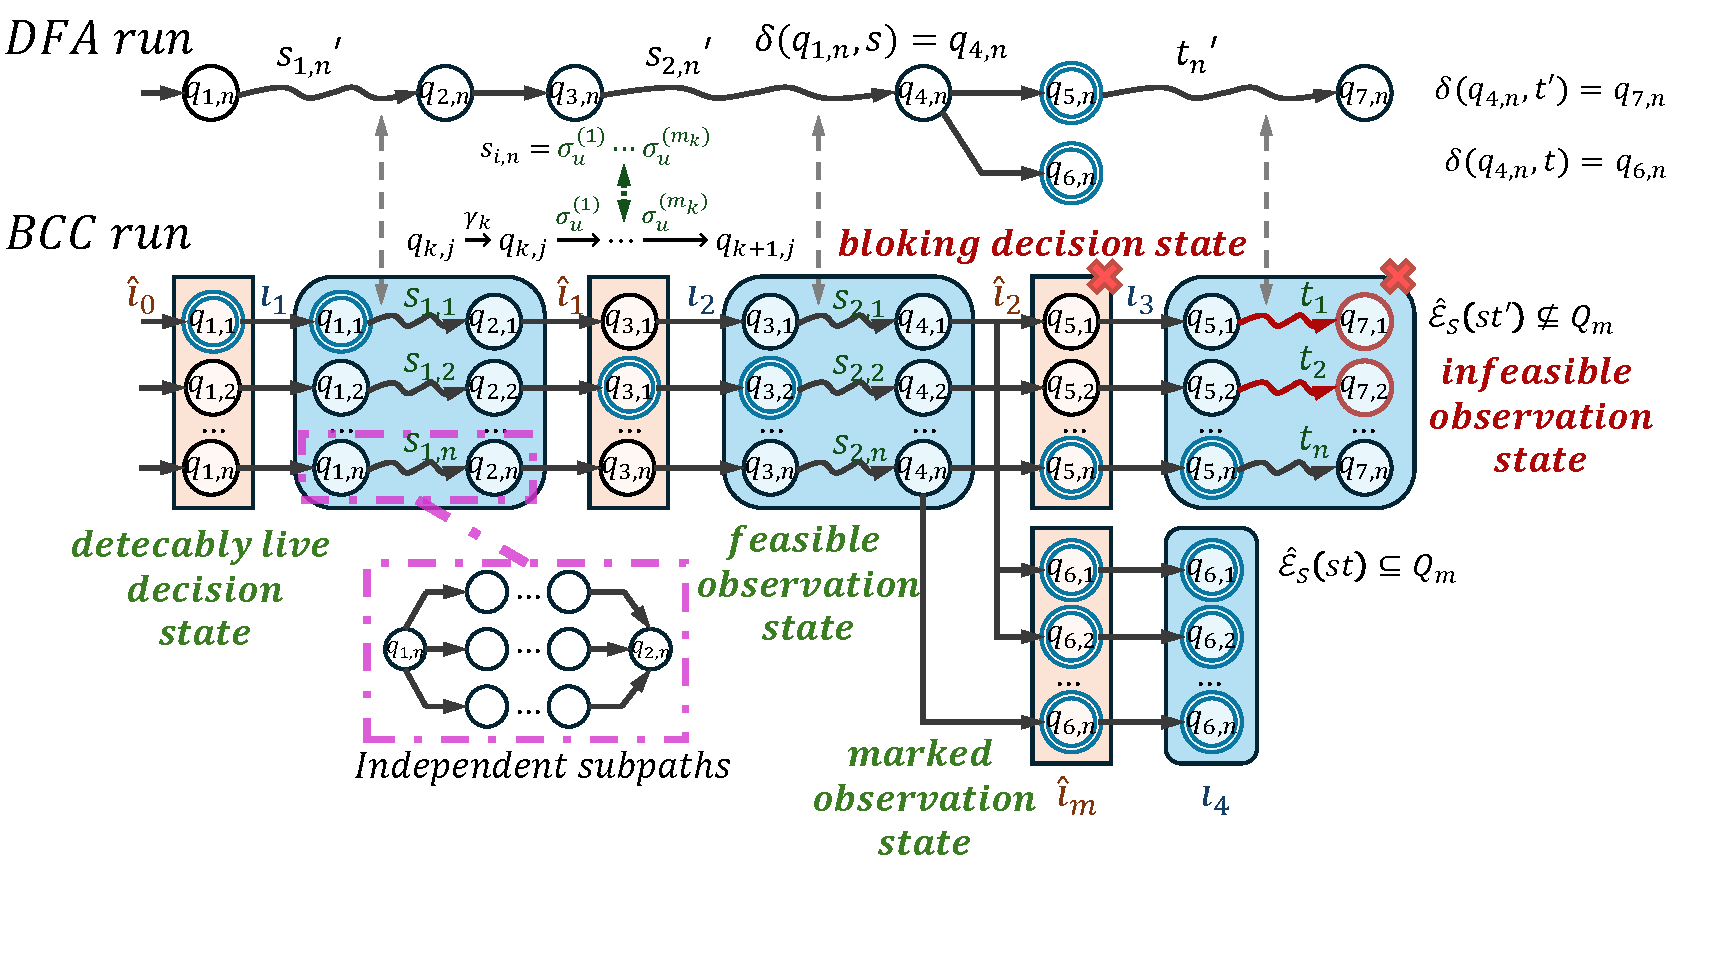
\includegraphics[width=0.625\linewidth]{Figs/conceptual_proof.pdf}
    % \caption{Conceptual illustration of the structural soundness in Theorem~\ref{theo:cnb}. 
    % For an arbitrary reachable state, a detectably live decision state admits a continuation to a marked decision state $\hat{\imath}_m \in \hat{\mathbb{I}}_m$, while a potentially feasible observation state admits an observable exit to such a live decision state. 
    % Red-crossed components indicate detectable-blocking or infeasible branches that are excluded from any IC-BTS satisfying Definitions~\ref{def:con_bcc}, \ref{def:z_pf}, and \ref{def:y_cl}.}
    \caption{Conceptual illustration of the correspondence between detectable non-blockingness and the structural properties of IC-BTS. 
    A run of the IC-BTS captures the evolution of the controlled DES at both the observation level and the DFA-state level. 
    A detectably non-blocking execution requires that every reachable state admits a path to a detectably marked decision state, where observation states along the path are potentially feasible, and decision states are detectably live. 
    Conversely, any IC-BTS representing a detectably non-blocking closed-loop system must preserve these properties and satisfy observation consistency. 
    The red-crossed components indicate branches violating potential feasibility, detectable liveness, or consistency, which cannot appear in a valid detectably non-blocking IC-BTS.}
    
    \label{fig:conceptual_proof}
\end{figure*}

\subsection{Synthesized supervisor and correctness}

In this subsection, we show how the detectably non-blocking IC-BTS $\mathfrak{S}$ induces a supervisor and establishes the correctness of the synthesis algorithm.
%
Recall that for a run $\rho$ of IC-BTS $\mathfrak{S}$ in the form of \eqref{eq:run_bcc}, the corresponding event sequence and control-pattern sequence are denoted as $\rho\restriction_{\sigma}$ and $\rho\restriction_{\gamma}$ in \eqref{eq:seq_bcc:sigma}, respectively.
% 
% 
% 下面改用leadsto
% Moreover, we have defined the transition function $\delta_{\mathfrak{S}} := \delta_{\mathfrak{S}} \cup \delta_{\mathfrak{S}} \cup \delta_{\mathfrak{S}}$.
% Following the definition of $\delta$, we extend $\delta_{\mathfrak{S}}: \mathcal{I} \times \Sigma_{\mathfrak{S}}^*$ recursively such that $\iota = \delta_{\mathfrak{S}}(\hat{\imath}_0, \rho\restriction_\delta)$, where $\Sigma_{\mathfrak{S}} = \Sigma \times \Gamma$.

%
We use $S_{\mathfrak{S}}$, which uses the historical evolution of IC-BTS, $\rho$, in place of the DFA-based supervisor 
$S: P(\mathcal{L}(G)) \rightarrow \Gamma$ to enforce detectable non-blockingness. 
For each observation sequence $\alpha \in P(\mathcal{L}_{\Sigma}(\mathfrak{S}))$, define
\begin{flalign}\label{eq:bcc_sc:1}
S_{\mathfrak{S}}(\alpha) = \gamma, \quad &\exists 
    \rho = \hat{\imath}_0 \xrightarrow{\gamma_0} \cdots \xrightarrow{\sigma_o} \hat{\imath} : \notag \\
&[\alpha = P(\rho\restriction_{\sigma})] \wedge [\delta_{DO}(\hat{\imath}, \gamma)!].
\end{flalign}
That is, $S_{\mathfrak{S}}$ returns the set of admissible control patterns $\gamma$ over all IC-BTS runs $\rho$ for which the observable event sequence is equal to $\alpha$.
%
The closed-loop language induced by $S_{\mathfrak{S}}$ is then defined by the event projections of the same IC-BTS runs
\begin{flalign}\label{eq:bcc_sc:1.5}
&\mathcal{L}(S_{\mathfrak{S}}/G) = \notag \\[-0.6em]
\{& s\in\Sigma^* \mid
\exists \rho = \hat{\imath}_0 \xrightarrow{\gamma_0} \cdots \xrightarrow{\sigma_o^{(k-1)}} \hat{\imath}_k \xrightarrow{\gamma_k} \hat{\imath}_k \xrightarrow{\sigma_u^{(k,1)}} \cdots
: \notag \\ 
&[s = \rho\restriction_{\sigma}] \ \wedge   
[\rho\restriction_{\gamma} = \gamma_0 \cdots \gamma_k : \gamma_k \in S_{\mathfrak{S}}(P(s))] \}.
\end{flalign}

% \begin{align}
% \mathcal{L}(S_{\mathfrak{S}}/G)
% = &\left\{ s\in\Sigma^* \,\middle\vert\,
% \begin{array}{@{}l@{}}
% \exists \rho =
% \hat{\imath}_0 \xrightarrow{\gamma_0} \cdots
% \xrightarrow{\sigma_o^{(k-1)}} \hat{\imath}_k \\
% \qquad\xrightarrow{\gamma_k} \imath_{k,1}
% \xrightarrow{\sigma_u^{(k,1)}} \cdots : \\
% [s = \rho\restriction_{\sigma}] \ \wedge \\
% [\rho\restriction_{\gamma} = \gamma_0\cdots\gamma_k, \\
% \gamma_k \in S_{\mathfrak{S}}(P(s))]
% \end{array}
% \right\}.
% \label{eq:bcc_sc:1.5}
% \end{align}

Note that the event sequence is admissible by the closed-loop system $S_{\mathfrak{S}} / G$ if the control pattern sequence extracted from its corresponding IC-BTS run is permitted by supervisor $S_{\mathfrak{S}}$.
%
By Proposition~\ref{prop:bcc_dfa_consistency}, every such projected event sequence is a feasible execution of the DFA $G$.
Hence, we can simplify \ref{eq:bcc_sc:1.5} as
\begin{equation}\label{eq:bcc_sc:2}
    \mathcal{L}(S_{\mathfrak{S}} / G) = \{ \rho\restriction_{\sigma} \in \Sigma^* \mid \forall \rho! \},
\end{equation}
and apply $S_\mathfrak{S}$ as $S$ such that $\mathcal{L}(S_{\mathfrak{S}} / G)$ can be used as an equivalent closed-loop representation of the controlled DES, $\mathcal{L}(S/G)$.
%
Now, we give the following two theorems to show the structural characterization of detectable non-blockingness. 
%
% Soundness of the algorithm
\begin{mythm}\label{theo:cnb}
Given a DFA $G = (Q, \Sigma, \delta, q_0, Q_m)$ and a corresponding IC-BTS
$
\mathfrak{S} = (\hat{\mathbb{I}}, \mathbb{I}, \hat{\imath}_0, \Sigma, \Gamma, \delta_{DO}, \delta_{OO}, \delta_{OD}),
$
suppose that all decision and observation states of ${\mathfrak{S}}$ are accessible from $\hat{\imath}_0$ and satisfy Definitions~\ref{def:con_bcc}, \ref{def:z_pf}, and \ref{def:y_cl}.
The supervisor $S$ induced by ${\mathfrak{S}}$ guarantees that the closed-loop system $S/G$ is detectable non-blocking.
\end{mythm}
%
\begin{pf}
The intuition of the proof is illustrated in Fig.~\ref{fig:conceptual_proof}. The proof consists of three steps.
First, we use the IC-BTS-DFA consistency to identify the closed-loop behavior $S/G$ with the event projection of the IC-BTS language.
Second, we show that the retained IC-BTS structure is detectably co-accessible to a marked decision macrostate.
Third, we show the observation consistency of the IC-BTS such that Definition~\ref{def:cnb} can be satisfied by the projected-back sequences.


By Proposition~\ref{prop:bcc_dfa_consistency} and \eqref{eq:bcc_sc:2} the closed-loop language generated by $S / G$ coincides with the event projection of the IC-BTS runs.
%
% Hence, for any IC-BTS run $\rho$ of the form \eqref{eq:run_bcc} satisfying
% $
%     \delta_{\mathfrak{S}}(\hat{\imath}_0, \rho\restriction_\delta) = \iota,
% $
% where $\rho\restriction_\delta$ is defined in \ref{eq:seq_bcc:delta} and $\iota$ equals to $(\hat{q}, \hat{x}) \in \hat{\mathbb{I}}$ or $(q, x, \gamma) \in \mathbb{I}$,
%
Hence, for any IC-BTS run $\rho$ of the form \eqref{eq:run_bcc} that originates at $\hat{\imath}_0$ and terminates at $\iota$, where $\iota$ is either $(\hat{q}, \hat{x}) \in \hat{\mathbb{I}}$ or $(q, x, \gamma) \in \mathbb{I}$, we have
$
    \delta(q_0, \rho\restriction_\sigma) = q,
$
in the original DFA $G$, where $\rho\restriction_\sigma$ is defined in \eqref{eq:seq_bcc:sigma}.


%
% TODO
% what is accessible, and what is co-accessible?
% not defined before
Now, we prove the detectably non-blocking condition on the IC-BTS and then project the result to the DFA.
%
Since $\mathfrak{S}$ is accessible, for an arbitrary state $\iota$, there exists a sequence $\tau_{q_0, q}$ in $\mathfrak{S}$ such that
$$
\hat{\imath}_0 \leadsto_{\mathcal{I}_f} \iota.
$$
Note that $\mathcal{I}_f$ denotes the union of the sets of detectably live decision states and potentially feasible observation states.
%
If $\iota$ is an observation state, then, according to Definition~\ref{def:z_pf}, there exists a successor decision state $\hat{\imath}'$ of $\iota$ such that
$
\iota \leadsto_{\mathcal{I}_f} \hat{\imath}'.
$
Moreover, according to Definition~\ref{def:y_cl}, we have
$$
\hat{\imath}' \leadsto_{\mathcal{I}_f} \hat{\imath}_m,
$$
where $\hat{\imath}_m$ denotes a detectably marked decision state that is accessible from $\hat{\imath}_0$.
%
If $\iota$ is a decision state, then we have
$$
\iota \leadsto_{\mathcal{I}_f} \hat{\imath}_m.
$$
Therefore, the detectably marked state $\hat{\imath}_m$ is reachable from $\iota$, and
the corresponding IC-BTS run $\rho$ from $\hat{\imath}_0$ to $\iota$ and ending at $\hat{\imath}_m$ can be projected back to DFA $G$ as $\rho\restriction_{\sigma}$.

Moreover, the bipartite structure preserves observation consistency among decision and observation states.
% 
Hence, for an arbitrary run $\rho'$ of the IC-BTS, if $\rho'$ is observation-equivariant with $\rho$, i.e., $P(\rho\restriction'_{\sigma}) = P(\rho\restriction_{\sigma})$, then based on the structural property of the IC-BTS, we have $\rho'\restriction_{X} = \rho\restriction_{X}$.
Therefore, the ending state of $\rho'$, $\hat{\imath}_m'$, must share the same detectably marked macrostate $\hat{x}_m$ with $\hat{\imath}_m$, such that this ending state is detectably marked.
Thus, the detectable state estimate induced by the observation $P(\rho\restriction_{\sigma})$ satisfies
%
\begin{flalign}\label{eq:pf:thm:1}
%\widehat{\bm{\mathcal{E}}}_{\mathfrak{S}}(P(st)) := 
\{ &q \in Q \mid 
\exists \rho' :  P(\rho\restriction'_{\sigma}) = P(\rho\restriction_{\sigma}), \notag \\
& \delta(q_0, \rho\restriction'_{\sigma}) = q \},
\end{flalign}
%
which is equal to $\hat{\mathcal{E}}_S(P(\rho\restriction_{\sigma})) $ in \eqref{eq:immed_esti}.
Since $\hat{\imath}_m'$ is detectably marked, \eqref{eq:pf:thm:1} is a subset of $Q_m$, which satisfies Definition~\ref{def:cnb}.
%
This completes the proof.
\end{pf}

% Soundness: 只要系统证明了某件事，那么这件事在语义上确实成立。
% Completeness: 只要某件事实际上成立，系统就一定能把它证明/表示出来。
\begin{mythm}\label{theo:cnb_complete}
Given a DFA $G = (Q, \Sigma, \delta, q_0, Q_m)$, suppose that the closed-loop system $S / G$ satisfies the notion of detectable non-blocking.
Then, the corresponding IC-BTS
$
\mathfrak{S} = (\hat{\mathbb{I}}, \mathbb{I}, \hat{\imath}_0, \Sigma, \Gamma, \delta_{DO}, \delta_{OO}, \delta_{OD}),
$
constructed for $S / G$ satisfies Definitions~\ref{def:con_bcc},
\ref{def:z_pf}, and~\ref{def:y_cl}.
\end{mythm}















\begin{pf}
By Definition~\ref{def:cnb}, for any $s \in \mathcal{L}(S / G)$ with $q = \delta(q_0, s)$, there exists a continuation $t$ such that $st \in (\Sigma^*\Sigma_o) \cap \mathcal{L}(S / G)$ and, for any $t' \in (\Sigma^*\Sigma_o) \cap \mathcal{L}(S / G)$,
\begin{equation}\label{eq:theo_comp:1}
    P(t') = P(st) \Rightarrow \delta(q_0, t') \in Q_m.
\end{equation}
%
We next examine how the reachable state $q$ appears in the corresponding evolution of macrostates.
If $q = q_0$, then $q$ belongs to the initial decision macrostate $\hat{x}_{0}$, which is accessible to the detectably marked state $\hat{\imath}_m$, and the following decision-macrostate argument applies directly.



For the case where $q \neq q_0$, by Proposition~\ref{prop:bcc_dfa_consistency}, there exists an IC-BTS run
$\rho = \hat{\imath}_0 \xrightarrow{} \cdots \iota \xrightarrow{} \cdots \hat{\imath}_m$ defined in \eqref{eq:run_bcc}, such that $\iota$ corresponds to $q$, and $\hat{\imath}_m$ corresponds to $q_m$ and is detectably marked.
%
First, suppose that the incoming transition of $q$ in $s$ is observable and can be written as $q' \xrightarrow[]{\sigma_o} q$.
%
Then, $q$ corresponds to the decision state $(\hat{q}, \hat{x})$, and there exists a predecessor observation macrostate $(x', \gamma)$ with $q' \in x'$ such that
$$
NX_{\sigma_o}(x') = \hat{x}.
$$
%
By \eqref{eq:theo_comp:1}, after the continuation $t$, all closed-loop executions observation-equivalent to $st$ end in marked states.
This guarantees the existence of the subsequence of $\rho$ from $\iota$, namely, $(\hat{q}, \hat{x})$, to $\hat{\imath}_m$.
Thus, $(\hat{q}, \hat{x})$ is detectably live, and Definition~\ref{def:y_cl} holds.

Second, suppose that the incoming transition of $q$ is unobservable and can be written as $q' \xrightarrow[]{\sigma_{u}} q$. Then there exists a decision state $(\hat{q}', \hat{x}')$ and a control pattern $\gamma$ such that
$$
x = UR_{\gamma}(\hat{x}').
$$
That is, $\iota = (q, x, \gamma)$ is an observation state.
%
In IC-BTS $\mathfrak{S}$, the observation-equivalent states can be denoted as $(q', x, \gamma)$, $\forall q'$.
By \eqref{eq:theo_comp:1}, all these states must be accessible to the macrostate of $\hat{\imath}_m$, and hence to the successor decision state within $\rho$.
%
Therefore, no reachable observation macrostate in $\mathfrak{S}$ contains such deadlock or livelock observation states, and Definition~\ref{def:z_pf} holds.

It remains to verify the consistency defined in Definition~\ref{def:con_bcc}.
Since every sequence of the controlled system $S / G$ is representable by IC-BTS $\mathfrak{S}$, and $\emptyset$ is an admissible control pattern, if $st$ ends at state $q$ via an observable event $\sigma_o$, then there exists a decision state $(q, \hat{x})$ corresponding to $q$, and a transition $(q, \hat{x}) \xrightarrow{\emptyset} (q, x, \emptyset)$, such that $(q, x, \emptyset)$ belongs to the successor observation macrostate of the decision macrostate $\hat{x}$.
Otherwise, if $st$ ends at state $q$ via an unobservable event $\sigma_u$, then there exists an observation state $\imath$ corresponding to $q$, such that there exists a predecessor decision of $\imath$.
%
Moreover, since ${\mathfrak{S}}$ is induced by the closed-loop behavior of a partial-observation supervisor, every reachable decision macrostate has at least one control decision selected by $S$.
For each reachable observation macrostate, every feasible observable event enabled by its control pattern must also be represented by a successor decision macrostate.
Otherwise, some possible closed-loop evolution under the same observation would be missing from $\mathfrak{S}$.
Hence, Definition~\ref{def:con_bcc} also holds.
%
Consequently, the IC-BTS constructed for the detectably non-blocking closed-loop system satisfies Definitions~\ref{def:con_bcc}, \ref{def:z_pf}, and~\ref{def:y_cl}.
\end{pf}

Intuitively, a closed-loop system is detectably non-blocking if and only if its behavior can be represented by an accessible IC-BTS satisfying consistency, potential feasibility, and detectable liveness.
%
The following corollary states the correctness of Algorithm~\ref{alg:cnb_syn}.
The algorithm returns a nonempty IC-BTS exactly when the detectably non-blocking synthesis problem is solvable.
If a nonempty IC-BTS remains after pruning, it directly induces a detectably non-blocking supervisor.
Conversely, if such a supervisor exists, then its closed-loop behavior admits an IC-BTS representation satisfying the same structural requirements, so the pruning procedure cannot eliminate all states.

\begin{mycol}\label{cor:alg_cnb_sound}
Algorithm~\ref{alg:cnb_syn} returns a nonempty IC-BTS rather than ``No solution'' if and only if there exists a partial-observation supervisor $S$ such that the closed-loop system $S/G$ is detectably non-blocking.
%
Moreover, if Algorithm~\ref{alg:cnb_syn} returns a nonempty IC-BTS $\mathfrak{S}$, then the supervisor $S_{\mathfrak{S}}$ induced by $\mathfrak{S}$ guarantees that $S_{\mathfrak{S}}/G$ is detectably non-blocking.
\end{mycol}



\begin{figure}[ht!]
    \centering
    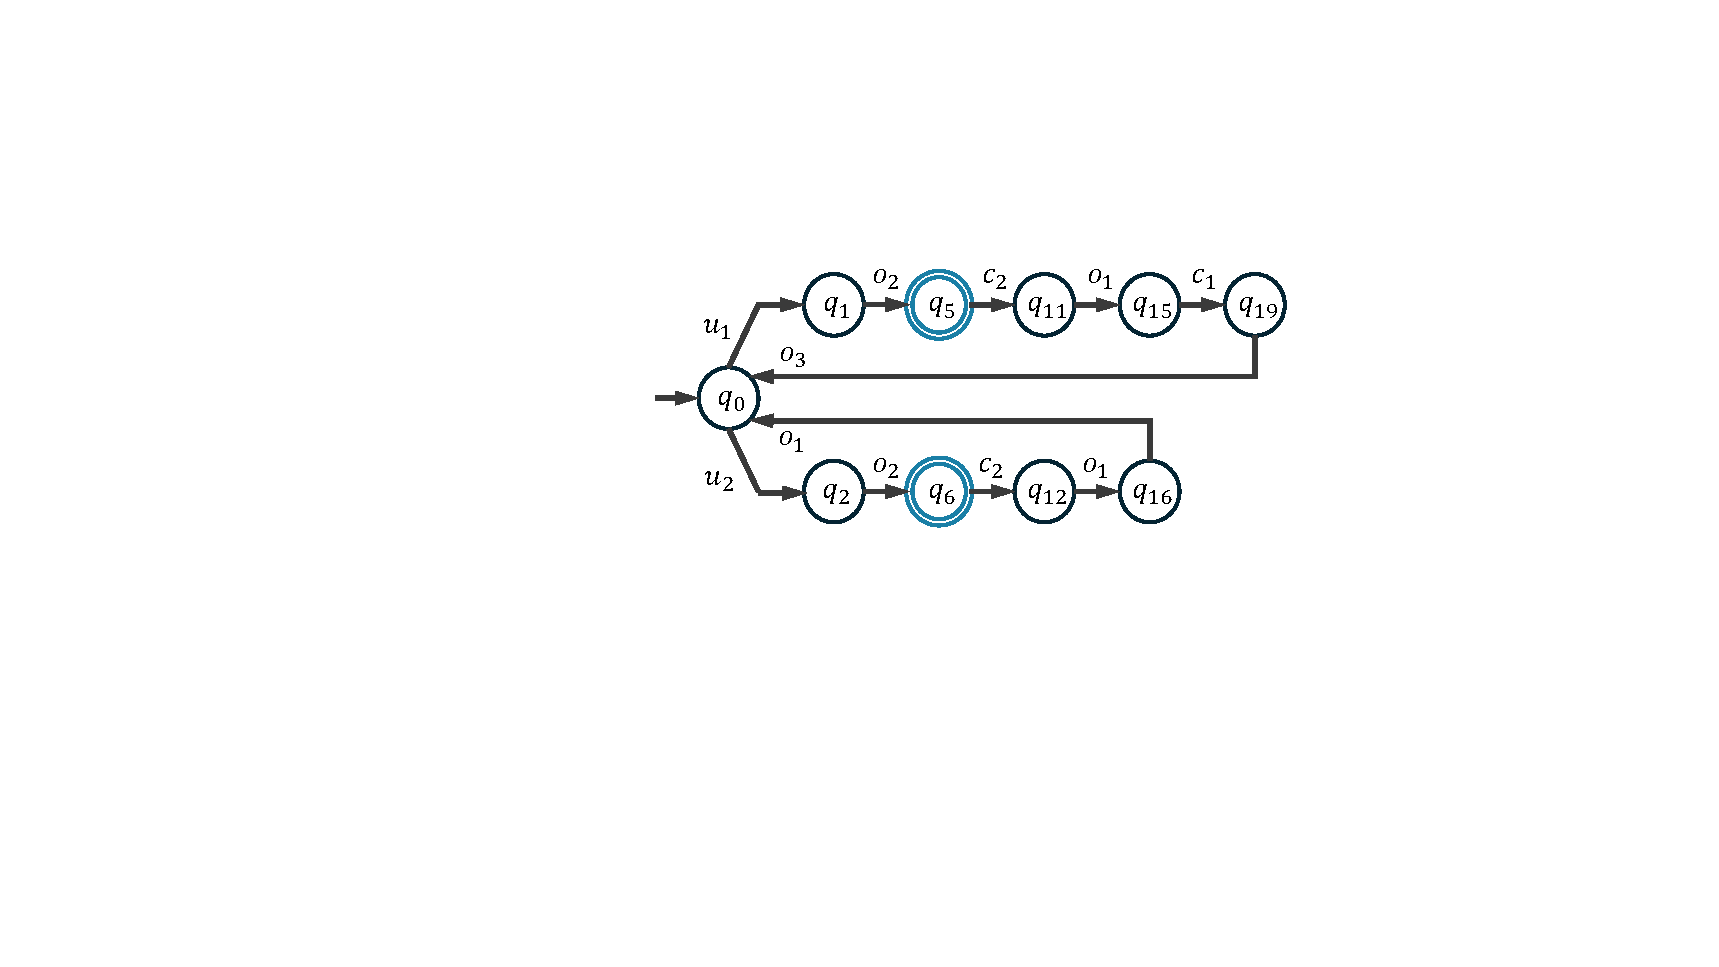
\includegraphics[width=0.65\linewidth]{Figs/controlled_fsa_overall.pdf}
    \caption{Controlled DFA $S / G$ from DFA $G$ in Fig.~\ref{fig:dfa_grid_env} and IC-BTS $\mathfrak{S}$ in Fig.~\ref{fig:bcc_overall}.}    % TODO 这个符号对不对
    \label{fig:ctrl_DFA}
\end{figure}

We give Example~\ref{ex:DFA_cnb} to illustrate that the closed-loop system satisfies the notion of detectable non-blockingness.
Meanwhile, we discuss the complexity of Algorithm~\ref{alg:cnb_syn}.

\begin{myexm}\label{ex:DFA_cnb}
    Let us consider the DFA illustrated in Fig.~\ref{fig:dfa_grid_env} (b) again, and the corresponding IC-BTS illustrated in Fig.~\ref{fig:bcc_overall}.
    %
    After pruning the inconsistent states, the corresponding closed-loop system $S / G$ is illustrated in Fig.~\ref{fig:ctrl_DFA}.
    %
    In the resulting closed-loop system, the evolutions from the initial state $q_0$ are $q_0 \xrightarrow{u_1} q_1 \xrightarrow{o_2} q_5$ and $q_0 \xrightarrow{u_2} q_2 \xrightarrow{o_2} q_6$, and the corresponding observation is $o_2$.
    In the detectable sense, after observing $o_2$, the supervisor can certify that the current DFA state belongs to the marked state set
    \begin{equation}\label{eq:ex_cnb_reach_marked}
        \hat{\mathcal{E}}_S(o_2) = \{ q_5, q_6 \} \subseteq Q_m,
    \end{equation}
    although the exact state may still be unknown.
    %
    Moreover, from any reachable state after $q_5$ or $q_6$, the controlled system can evolve through a finite admissible continuation and return to $q_0$.
    The particular observable labels along this return segment are not essential for the detectably non-blocking argument.
    After returning to $q_0$, the continuation for states of \eqref{eq:ex_cnb_reach_marked} can be applied again to reach the detectably marked information state $\{ q_5, q_6 \}$.
    %
    Hence, for any sequence in $G$ corresponding to a detectably live path in the IC-BTS $\mathfrak{S}$, there exists a continuation that reaches a detectably marked state.
    Once the supervisor $S$ is induced from the IC-BTS $\mathfrak{S}$ as described in Section~\ref{subsec:supervisor_induction}, the closed-loop system $S/G$ inherits this property and satisfies detectable non-blocking.

    % TODO
    % Let us consider the motivating example again in Section~\ref{sec:intro}.
    % The robotic system cannot certify its exact current state, but its state estimate can be updated after completing certain motion primitives.
    % When it is at the initial state $q_0$, it should reject the motions corresponding to $o_3$, which may lead to $q_3$ or $q_4$.
    % In this sense, it can then arrive at $q_5$ or $q_6$; moreover, when it observes the information corresponding to event $o_2$, it knows that it is in a safe location, so the transmission of critical information can be started.
\end{myexm}


% \begin{mypro}
% Consider an IC-BTS $\mathfrak{S}$ constructed over a DFA $G$ with the number of $|Q|$ states and $|\Sigma|$ events. 
% The worst-case time complexity of Algorithm~\ref{alg:cnb_syn} is
% $
%     O(|Q|\cdot |\Sigma|\cdot 2^{2|Q|+2|\Sigma|}).
% $
% \end{mypro}
%
% \begin{pf}
% Algorithm~\ref{alg:cnb_syn} proceeds by pruning decision and observation macrostates of the IC-BTS.
% In Lines 1--2, deadlock and livelock observation state are identified by a BFS
% search, which can be done in time
% $
% O(|Y + Z|+|\delta_{\mathfrak{S}}|)
% $.
% %
% In Lines 3--6, each iteration prunes decision macrostates that are not detectably live
% or observation macrostates that violate consistency. Each iteration can be implemented by one BFS over the remaining IC-BTS, with cost
% $
% O(|Y + Z|+|\delta_{\mathfrak{S}}|)
% $.
% Since each nontrivial iteration prunes at least one decision macrostate or observation macrostate, the
% number of iterations is at most $|W^Y|+|W^Z|$. Therefore, the total cost is
% $
%     O((|W^Y|+|W^Z|)(|Y + Z|+|\delta_{\mathfrak{S}}|)).
% $
% Line 7 performs one additional BFS, which is dominated by the above term.
% Hence, the overall complexity is
% $
%     O((|W^Y|+|W^Z|)(|Y + Z|+|\delta_{\mathfrak{S}}|)).
% $
% %
% %By Proposition~\ref{prop:state_bcc}, we have
% By \eqref{eq:prop:bcc:1} and \eqref{eq:prop:bcc:2}, we have
% $
%     |Y + Z|
%     \le
%     |Q|(2^{|Q|}+2^{|Q|+|\Sigma|})
%     =
%     O(|Q|\cdot 2^{|Q|+|\Sigma|}),
% $
% and
% $$
%     |\delta_{\mathfrak{S}}|
%     \le
%     |Q|2^{|Q|+|\Sigma|}(1+|\Sigma|)
%     =
%     O(|Q|\cdot |\Sigma|\cdot 2^{|Q|+|\Sigma|}).
% $$
% Therefore, based on
% $
% |W^Y|+|W^Z| = O(2^{|Q|+|\Sigma|}),
% $
% we have
% $$
% \begin{aligned}
%     O((|W^Y|+|W^Z|)(|Y + Z|+|\delta_{\mathfrak{S}}|))
%     &=
%     O(
%     2^{|Q|+|\Sigma|}
%     \cdot
%     |Q|\cdot |\Sigma|\cdot 2^{|Q|+|\Sigma|}
%     ) \\
%     &=
%     O(|Q|\cdot |\Sigma|\cdot 2^{2|Q|+2|\Sigma|}).
% \end{aligned}
% $$
% This completes the proof.
% \end{pf}
%

The pruning-based synthesis procedure in Algorithm~\ref{alg:cnb_syn} is exponential in both the state space and the event alphabet of the underlying DFA.
Its worst-case computational complexity is given by
$O(|Q|\cdot |\Sigma|\cdot 2^{2|Q|+2|\Sigma|})$, where $|Q|$ is the number of states, and $|_\Sigma|$ is the number of events.

As for the maximally permissiveness of the synthesized supervisor, the comparison of control patterns should be made at the same decision instant. 



Consider the macrostate sequence $\rho\restriction_X$ defined in \eqref{eq:seq_bcc:X}, which is synthesized by supervisor \eqref{eq:bcc_sc:1}.
The maximally permissiveness requires that for all $\gamma_i$ defined in $(x_i, \gamma_i)$, we have for any other $\gamma_i'$ defined in $x_i$, we have $\gamma_i \not \subset \gamma_i'$.
In this sense, the maximally permissive partial-observation supervisor can be defined as
%
\begin{flalign}\label{eq:mps_cnb}
S_{\mathfrak{S}}(\alpha) = \gamma, \quad  &\exists 
    \rho = \hat{\imath}_0 \xrightarrow{\gamma_0} \cdots \xrightarrow{\sigma_o} \hat{\imath}, \notag \\
    & \alpha = P(\rho\restriction_{\sigma}) : 
      [\delta_{DO}(\hat{\imath}, \gamma)!] \wedge \notag \\
    &[\nexists \gamma' \in \Gamma : \delta_{DO}(\hat{\imath}, \gamma')! \wedge \gamma \subset \gamma'] \}.
\end{flalign}

\begin{mycol}
Problem~\ref{prob:cnb} can be solved within finite steps by Algorithm~\ref{alg:cnb_syn}, and the maximally permissive supervisor can be obtained from \eqref{eq:mps_cnb}.
\end{mycol}


\section{Special case: marked tasks within the unobservable reaches}
\label{sec:special_z_marked}

%
% 这个系统要处理的话
% 其实方法是一样的
% 1 对于marked observation state，需要当前Z-状态中的所有状态能够到达这个状态，或者退到下一个Y状态
% 2 Y状态不变
% 3 系统要consistent
% 

In this section, we discuss a special case of the proposed method, namely, systems in which marked tasks may be completed within unobservable reaches.
In the previous sections, detectable non-blockingness is formulated based on the certification of marked states after observation updates.
This formulation is consistent with the physical interpretation that task completion should be certified from the observation.
However, from a mathematical perspective, this requirement can be restrictive when a marked state is reached within an unobservable evolution before the next observable event occurs.
%
To cover this situation, we extend the notion of detectable non-blockingness by allowing task completion to be certified even if the marked state is visited within the preceding unobservable reach, and the formal definition is given as follows
\begin{equation}
    \forall s \in \mathcal{L}(S/G), \exists t \in \Sigma^* : \mathcal{E}_S(st) \subseteq Q_m.
\end{equation}

Under this formulation, the detectably marked states are naturally defined over decision states, since decision states represent those unobservable states immediately after observation updates.
However, in some systems, a marked state can be reached inside an observation state before the next observable event occurs.
%
The main result of this article already handles the case where task completion is certified at marked decision states. Therefore, we only briefly discuss the case of marked observation states here.

To handle this case, we extend the target state set of the IC-BTS by including detectably marked observation states, which are formally defined as $\mathbb{I}_{m}(x_m, \gamma)$, where $x_{m} \subseteq Q_m$.
Meanwhile, the set of exit observation states can be defined as
$$
\begin{aligned}
    \mathbb{I}_{e} =
    \{ &(q_e, x_e, \gamma) \in \mathbb{I} \mid
    \exists \sigma_o \in \Sigma_o : \\
       &\delta_{OD}((q_e, x_e, \gamma), \sigma_o)! \wedge \delta(q_e,\sigma_o)! \}.        
\end{aligned}
$$
%
Given a detectably marked observation state $(q_m, x_m, \gamma)$, if its corresponding marked marcostate $(x_m, \gamma)$ must satisfy
\begin{enumerate}[(i)]
    \item for every observation state $\imath = (q, x_m, \gamma)$, there exists a marked observation state $\imath_m$ within $\mathbb{I}(x_m, \gamma)$, such that
    $$
        \imath \leadsto_{\mathbb{I}(x_m,\gamma)} \imath_m.
    $$

    \item for the marked observation state $\imath_m$ in (i), every path originating from $\imath_m$ and inside $\mathbb{I}(x_m,\gamma)$ must end with an exit observation state $\imath_e \in \mathbb{I}_{e}$, that is, for every state sequence
    $$
        \rho\restriction_{\imath} = \imath_{i,0} \ \imath_{i,1} \ \cdots \ \imath_{i,j} \ \cdots \ \imath_{i,\ell},
    $$
    $\imath_{i,0} = \imath_m, \, \imath_{i,\ell} = (q_e, x_e, \gamma)$, we have
    $
        \imath_{i,j} \leadsto_{\mathbb{I}(x_m,\gamma)} \imath_{k,e},
    $
    with $i = 0, \ldots , \ell - 1$, $j,k \in \mathbb{N}$.
\end{enumerate}
%
Hence, after reaching the marked observation state $\imath_m$, all subsequent internal evolution inside $\mathbb{I}(x_m,\gamma)$ can eventually reach an exit observation state $\imath_{k,e}$.
%
Thus, the observed exit can certify task completion within the unobservable reach.

Then, the target set for detectable-liveness is extended from
$\hat{\mathbb{I}}_m$ to
\begin{equation}\label{eq:extended_target_set}
\mathcal{I}_m
= \hat{\mathbb{I}}_m \cup \bigcup_{(x_m, \gamma)} \mathbb{I}(x_m,\gamma),
\end{equation}
Accordingly, the definition of detectably live decision macrostates $\iota$, which now equals to $\hat{x}$ or $(x, \gamma)$, in Definition~\ref{def:y_cl} can be extended by redefining the macrostate sequence $\rho\restriction_{X}$ within as
\begin{equation}\label{eq:bcc_y_cl:2}
    \hat{x} (x_{k+1}, \gamma_{k+1}) \hat{x}_{k+1} (x_{k+2}, \gamma_{k+2}) \cdots (x_{k+i}, \gamma_{k+i}) \hat{x}_m,    
\end{equation}
or
\begin{equation}\label{eq:bcc_y_cl:3}
    (x, \gamma) \hat{x}_{k+1} (x_{k+1}, \gamma_{k+1}) \hat{x}_{k+2} \cdots (x_{k+i}, \gamma_{k+i}) \hat{x}_m,    
\end{equation}
Thus, a detectably live decision state is allowed to reach either a decision state or an observation state, which is detectably marked, with an internal path to the next observable exit.
%
Based on these modifications, Algorithm~\ref{alg:cnb_syn} can still be applied to obtain a consistent IC-BTS. 
The resulting IC-BTS then induces a detectably non-blocking supervisor for systems in which task completion can be certified either at marked decision states or within marked observation states, thereby solving Problem~\ref{prob:cnb}.

% It should be noted that completion of a marked observation state is certified only after the subsequent observable exit is observed. 
% This is sufficient for the mathematical definition, since all compatible IC-BTS paths must have visited a marked observation state before the exit. 
% However, in many practical applications, the unobservable tail inside the observation state is not physically observed, and thus the exact occurrence of task completion may not be directly interpretable from the subsequent observation alone.


% ---------------------------------------------------------------------------

\section{Conclusion}\label{sec:con}
%
In this article, we proposed a new non-blocking property, called detectable non-blocking, under which the observer can certify that the system is able to reach a marked state. 
Based on this notion, we developed a supervisor synthesis algorithm that constructs a controlled sublanguage guaranteed to be detectable non-blocking. 
We also proved that the proposed synthesis algorithm terminates in finite steps. 
%
Future work will investigate how the notion of detectable non-blocking can be extended to weighted and interval-weighted systems, where task completion may depend not only on reachability but also on accumulated transition weights.


\bibliographystyle{plain}
\bibliography{ref_full}
\end{document}